%%%%%%%%%%%%%%%%%%%%%%%%%%%%%%%%%%%%%%%%%
% Beamer Presentation
% LaTeX Template
% Version 1.0 (10/11/12)
%
% This template has been downloaded from:
% http://www.LaTeXTemplates.com
%
% License:
% CC BY-NC-SA 3.0 (http://creativecommons.org/licenses/by-nc-sa/3.0/)
%
%%%%%%%%%%%%%%%%%%%%%%%%%%%%%%%%%%%%%%%%%

%----------------------------------------------------------------------------------------
%	PACKAGES AND THEMES
%----------------------------------------------------------------------------------------

\documentclass[serif]{beamer}

\mode<presentation>{
	
	% The Beamer class comes with a number of default slide themes
	% which change the colors and layouts of slides. Below this is a list
	% of all the themes, uncomment each in turn to see what they look like.
	
	%\usetheme{default}
	%\usetheme{AnnArbor}
	%\usetheme{Antibes}
	%\usetheme{Bergen}
	%\usetheme{Berkeley}
	%\usetheme{Berlin}
	%\usetheme{Boadilla}
	%\usetheme{CambridgeUS}
	%\usetheme{Copenhagen}
	%\usetheme{Darmstadt}
	%\usetheme{Dresden}
	%\usetheme{Frankfurt}
	%\usetheme{Goettingen}
	%\usetheme{Hannover}
	%\usetheme{Ilmenau}
	%\usetheme{JuanLesPins}
	%\usetheme{Luebeck}
	\usetheme{Madrid}
	%\usetheme{Malmoe}
	%\usetheme{Marburg}
	%\usetheme{Montpellier}
	%\usetheme{PaloAlto}
	%\usetheme{Pittsburgh}
	%\usetheme{Rochester}
	%\usetheme{Singapore}
	%\usetheme{Szeged}
	%\usetheme{Warsaw}
	
	% As well as themes, the Beamer class has a number of color themes
	% for any slide theme. Uncomment each of these in turn to see how it
	% changes the colors of your current slide theme.
	
	%\usecolortheme{albatross}
	\usecolortheme{beaver}
	%\usecolortheme{beetle}
	%\usecolortheme{crane}
	%\usecolortheme{dolphin}
	%\usecolortheme{dove}
	%\usecolortheme{fly}
	%\usecolortheme{lily}
	%\usecolortheme{orchid}
	%\usecolortheme{rose}
	%\usecolortheme{seagull}
	%\usecolortheme{seahorse}
	%\usecolortheme{whale}
	%\usecolortheme{wolverine}
	
	%Some nicer color definitions
	\definecolor{crimsonred}{RGB}{153,0,0}		% Neurtal red, good for dark or light bg
	\definecolor{darkcharcoal}{RGB}{25,25,25}		% Darker gray
	\definecolor{charcoal}{RGB}{51,51,51}		% Darker gray
	\definecolor{ash}{RGB}{100,100,100}			% medium gray
	\definecolor{paleblue}{RGB}{0,102,102}		% More of an `ocean' color
	\definecolor{turtlegreen}{RGB}{51,153,0}	% A more neutral green
	\definecolor{paleale}{RGB}{204,204,102}		% Only for dark BG
	\definecolor{lager}{RGB}{140,110,10}		% Use instead of pale ale for white BG
	\definecolor{regal}{RGB}{90,0,120}			% A more neutral purple
	\definecolor{jeans}{RGB}{20,30,150}			% A more neutral blue
	\definecolor{Alert}{RGB}{51,153,0}	
	
	
	\setbeamercolor{block title}{bg=red!30,fg=black}
	
	%\setbeamertemplate{footline} % To remove the footer line in all slides uncomment this line
	%\setbeamertemplate{footline}[page number] % To replace the footer line in all slides with a simple slide count uncomment this line
	
	%\setbeamertemplate{navigation symbols}{} % To remove the navigation symbols from the bottom of all slides uncomment this line
}

\small
\usepackage{graphicx} % Allows including images
\usepackage{palatino}
\usepackage{colortbl}

\usepackage[minnames=2,maxnames=3,style=numeric,backend=bibtex,sorting=none]{biblatex}
\addbibresource{bib/mybib}

\newcommand {\e}[1]{\mathrm{~#1}}
\newcommand {\E}[1]{\times 10^{#1}}

\newcommand{\backupbegin}{
	\newcounter{finalframe}
	\setcounter{finalframe}{\value{framenumber}}
}
\newcommand{\backupend}{
	\setcounter{framenumber}{\value{finalframe}}
}

\setlength{\extrarowheight}{.8ex}

\usepackage{tikz}
\usepackage{amsmath}
\usepackage{verbatim}
\usetikzlibrary{arrows,shapes}
\usetikzlibrary{fadings}
\usetikzlibrary{tikzmark}

\renewcommand{\thefootnote}{\fnsymbol{footnote}}

\usepackage{booktabs} % Allows the use of \toprule, \midrule and \bottomrule in tables

\definecolor{darkgreen}{rgb}{0.0, 0.5, 0.0}
\setbeamertemplate{navigation symbols}{} %remove navigation symbols

\newcommand{\putat}[3]{\begin{picture}(0,0)(0,0)\put(#1,#2){#3}\end{picture}}


% Python listing setup

\usepackage{color}
\usepackage[procnames]{listings}
\usepackage{textcomp}
\usepackage{setspace}
\usepackage{palatino}
\renewcommand{\lstlistlistingname}{Code Listings}
\renewcommand{\lstlistingname}{Code Listing}
\definecolor{gray}{gray}{0.5}
\definecolor{green}{rgb}{0,0.5,0}
\definecolor{lightgreen}{rgb}{0,0.7,0}
\definecolor{purple}{rgb}{0.5,0,0.5}
\definecolor{darkred}{rgb}{0.5,0,0}
\lstnewenvironment{python}[1][]{
\lstset{
language=python,
basicstyle=\ttfamily\footnotesize\setstretch{1},
stringstyle=\color{green},
showstringspaces=false,
alsoletter={1234567890},
otherkeywords={\ , \}, \{},
keywordstyle=\color{blue},
emph={access,and,as,break,class,continue,def,del,elif,else,%
except,exec,finally,for,from,global,if,import,in,is,%
lambda,not,or,pass,print,raise,return,try,while,assert},
emphstyle=\color{orange}\bfseries,
emph={[2]self},
emphstyle=[2]\color{gray},
emph={[4]ArithmeticError,AssertionError,AttributeError,BaseException,%
DeprecationWarning,EOFError,Ellipsis,EnvironmentError,Exception,%
False,FloatingPointError,FutureWarning,GeneratorExit,IOError,%
ImportError,ImportWarning,IndentationError,IndexError,KeyError,%
KeyboardInterrupt,LookupError,MemoryError,NameError,None,%
NotImplemented,NotImplementedError,OSError,OverflowError,%
PendingDeprecationWarning,ReferenceError,RuntimeError,RuntimeWarning,%
StandardError,StopIteration,SyntaxError,SyntaxWarning,SystemError,%
SystemExit,TabError,True,TypeError,UnboundLocalError,UnicodeDecodeError,%
UnicodeEncodeError,UnicodeError,UnicodeTranslateError,UnicodeWarning,%
UserWarning,ValueError,Warning,ZeroDivisionError,abs,all,any,apply,%
basestring,bool,buffer,callable,chr,classmethod,cmp,coerce,compile,%
complex,copyright,credits,delattr,dict,dir,divmod,enumerate,eval,%
execfile,exit,file,filter,float,frozenset,getattr,globals,hasattr,%
hash,help,hex,id,input,int,intern,isinstance,issubclass,iter,len,%
license,list,locals,long,map,max,min,object,oct,open,ord,pow,property,%
quit,range,raw_input,reduce,reload,repr,reversed,round,set,setattr,%
slice,sorted,staticmethod,str,sum,super,tuple,type,unichr,unicode,%
vars,xrange,zip},
emphstyle=[4]\color{purple}\bfseries,
upquote=true,
morecomment=[s][\color{lightgreen}]{"""}{"""},
commentstyle=\color{red}\slshape,
literate={>>>}{\textbf{\textcolor{darkred}{>{>}>}}}3%
         {...}{{\textcolor{gray}{...}}}3,
procnamekeys={def,class},
procnamestyle=\color{blue}\textbf,
framexleftmargin=1mm, framextopmargin=1mm, frame=shadowbox,
rulesepcolor=\color{blue},#1
}}{}


%----------------------------------------------------------------------------------------
% & TITLE PAGE
%----------------------------------------------------------------------------------------

\title[$B \to K K \ell \nu_\ell$ decays @ Belle]{Study of $B \to K K \ell \nu_\ell$ Decays at Belle} % The short title appears at the bottom of every slide, the full title is only on the title page


\author[Matic Lubej]{Matic Lubej} % Your name
\institute[] % Your institution as it will appear on the bottom of every slide, may be shorthand to save space
{\large\underline{PhD Thesis Defense} \\ % Occasion for the title page
	\medskip
	%\textit{matic.lubej@ijs.si} % Your email address
}
\date[Ljubljana, November $22^{\mathrm{nd}}$, 2018]{Ljubljana, November $22^{\mathrm{nd}}$, 2018} % Date, can be changed to a custom date


\usebackgroundtemplate{
%	\tikz[overlay,remember picture] 
%	\node[opacity=0.2] (label) at (9.2,-6.5){
%	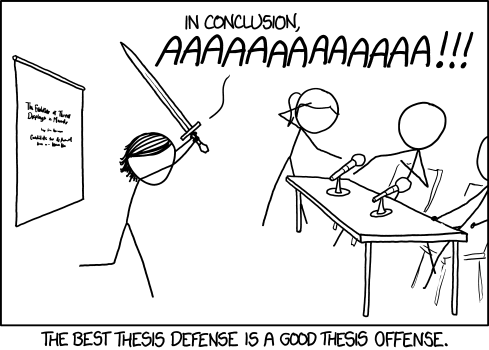
\includegraphics[scale=0.4]{fig/thesis_defense}
%	};
\tikzfading[name=fade out,
inner color=transparent!20,
outer color=transparent!99]
%Now we use the fading in another picture:
\begin{tikzpicture}[remember picture, overlay]
\node[opacity=1.0,inner sep=0pt, scope fading=fade out] at (11,-8)
{\scalebox{-1}[1]{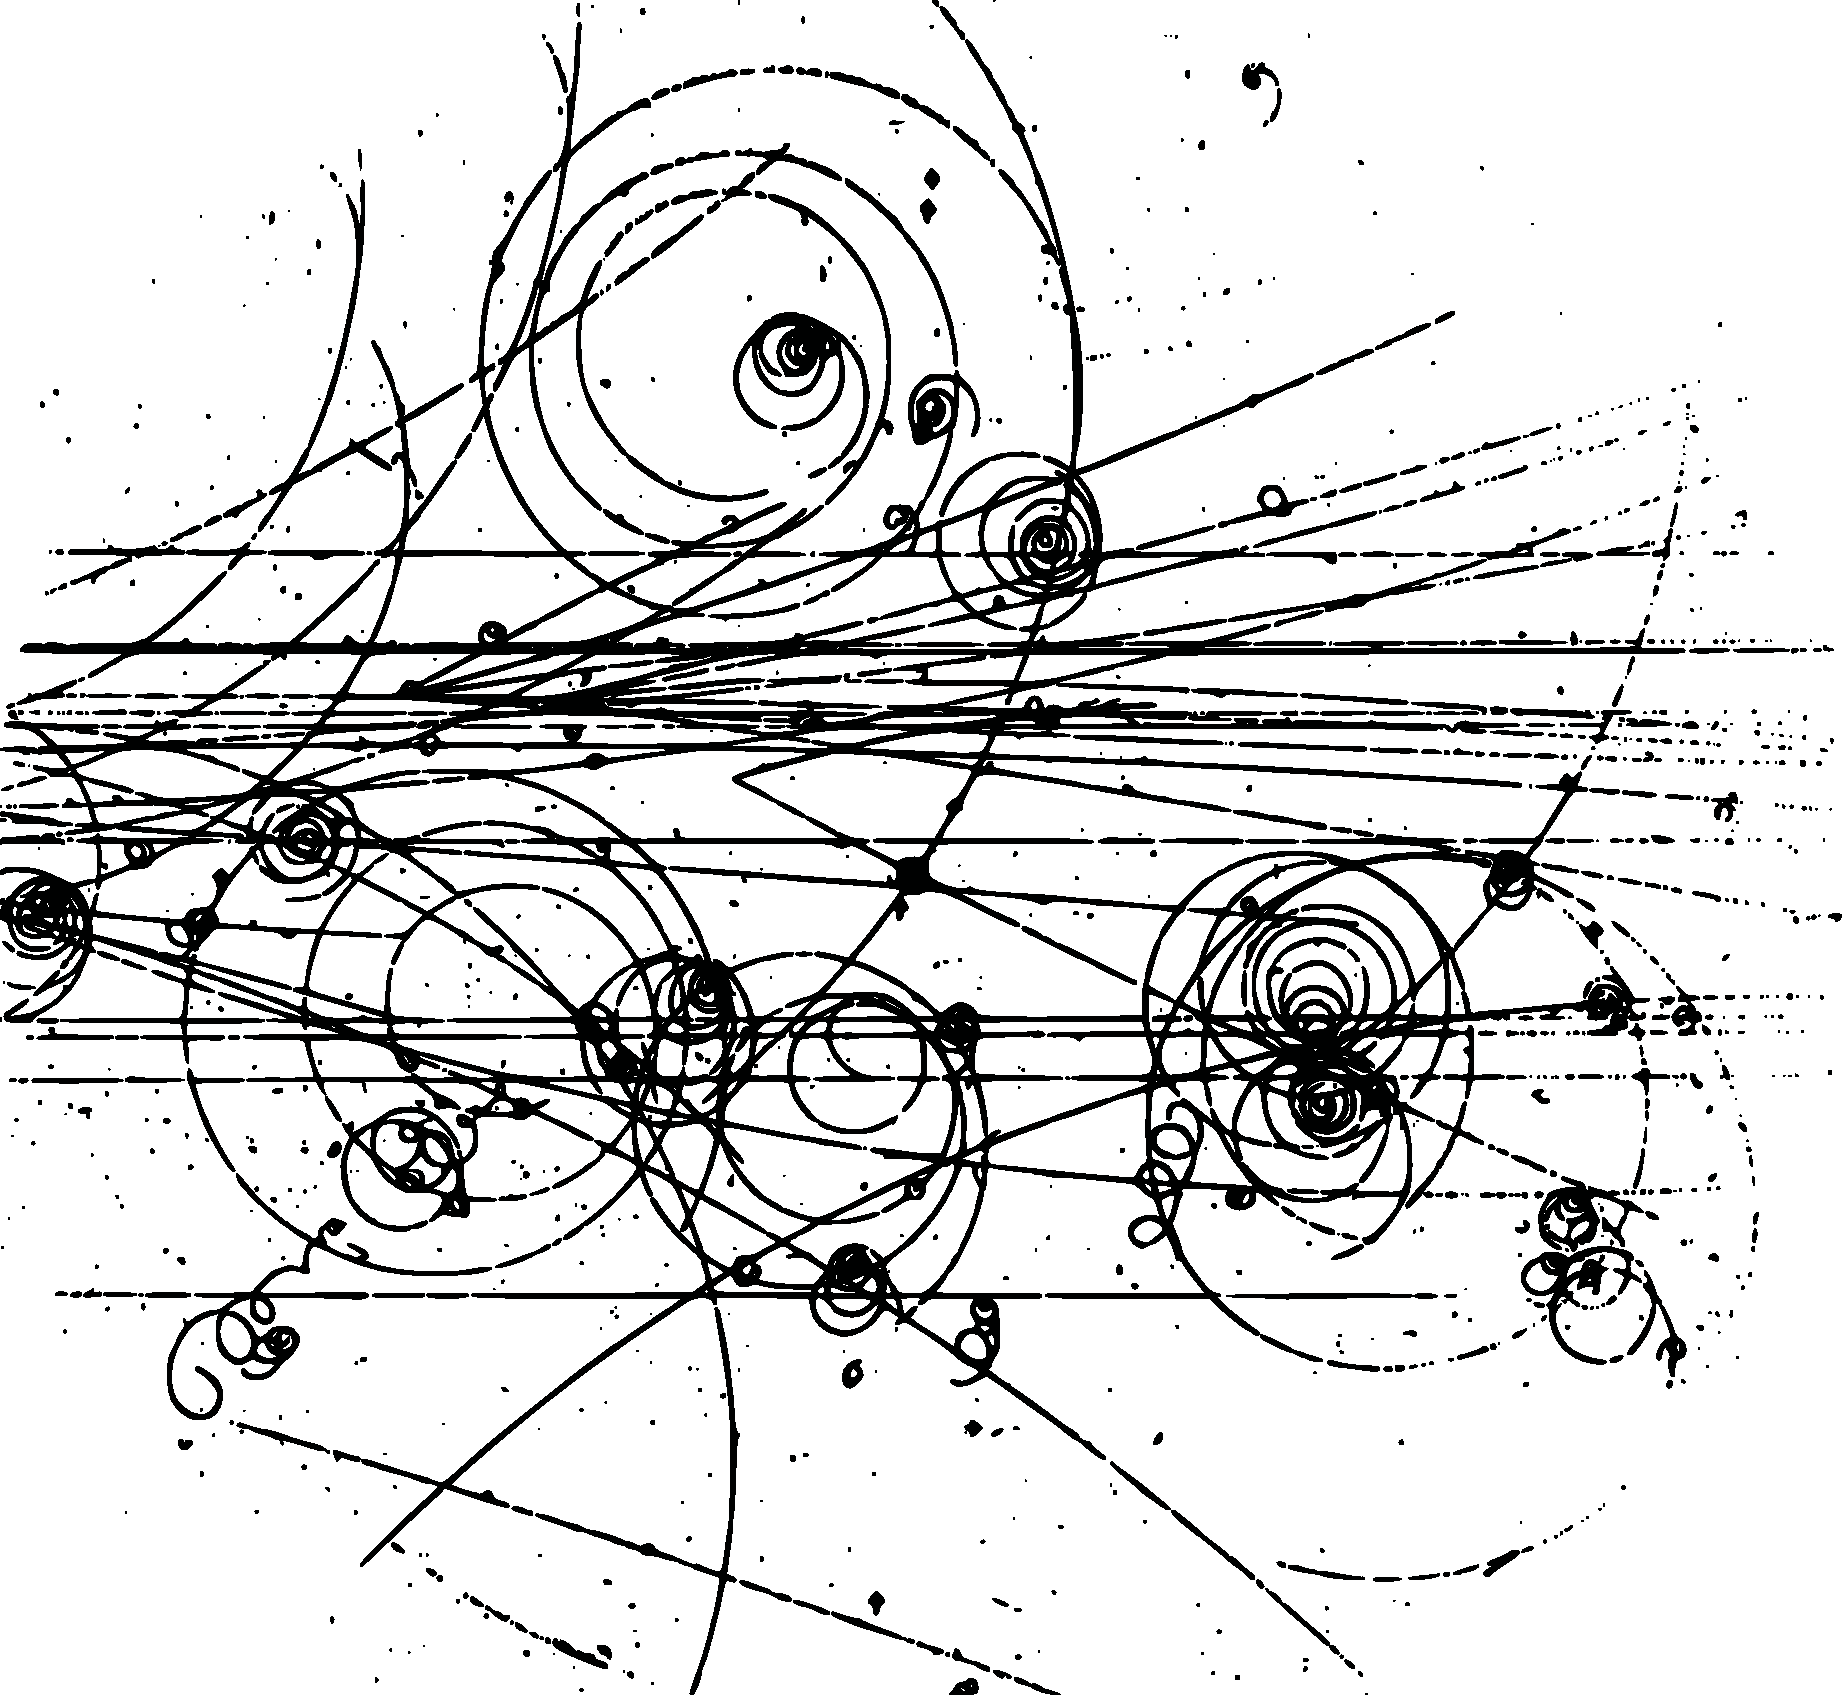
\includegraphics[width=0.6\linewidth]{fig/bc_1}}};
\end{tikzpicture}
}

\begin{document}
	
	\begin{frame}
	\frametitle{}
	\thispagestyle{empty}
	\begin{center}
		\putat{-120}{-30}{
\includegraphics[height=1.5cm]{fig/b2logo}}
		\putat{-40}{-30}{
\includegraphics[height=2cm]{fig/fmflogo}}
		\putat{80}{-30}{
\includegraphics[height=1.5cm]{fig/ijslogo}}
		\putat{103}{-30}{IJS}
		
	\end{center}

%\tikzfading[name=fade out,
%inner color=transparent!0,
%outer color=transparent!90]
%%Now we use the fading in another picture:
%\begin{tikzpicture}[remember picture, overlay]
%\node[opacity=1.0,inner sep=0pt, scope fading=fade out] at (1,-6)
%{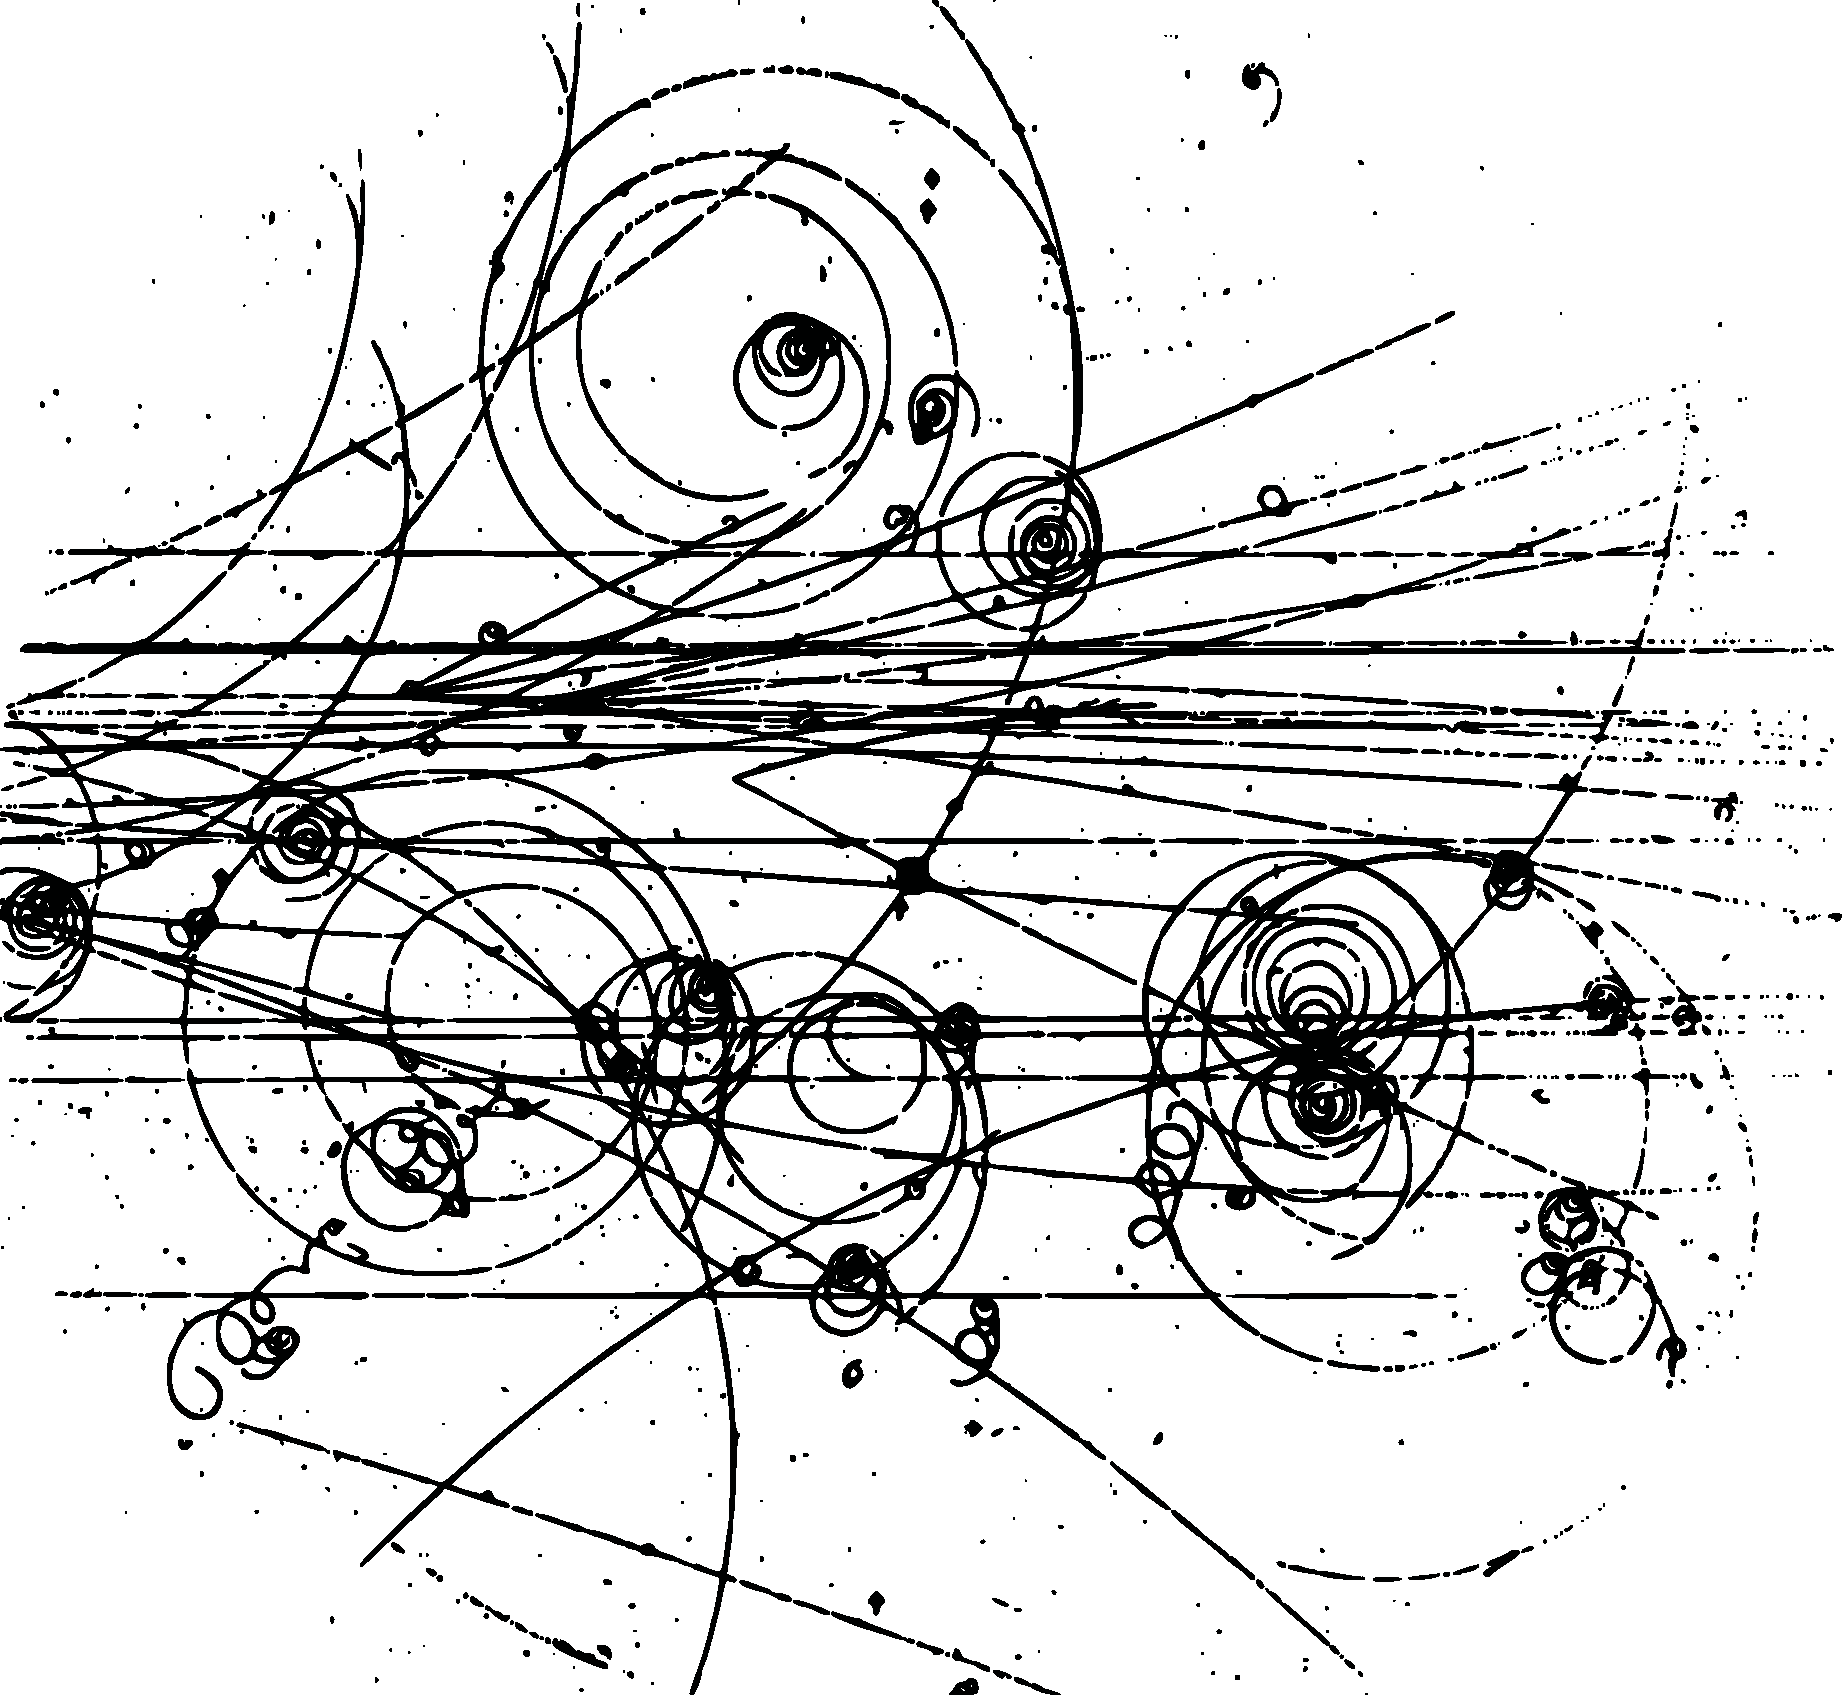
\includegraphics[width=0.6\linewidth]{fig/bc_1}};
%\end{tikzpicture}


	\maketitle
\end{frame}

%----------------------------------------------------------------------------------------

%\usebackgroundtemplate{}

\usebackgroundtemplate{
	%	\tikz[overlay,remember picture] 
	%	\node[opacity=0.2] (label) at (9.2,-6.5){
	%	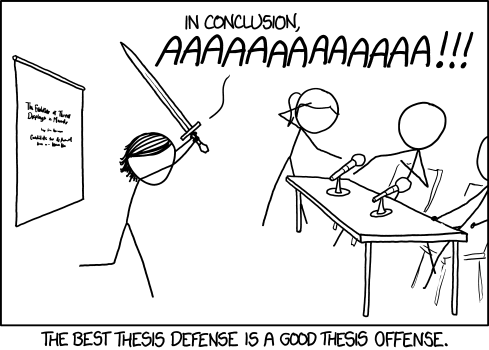
\includegraphics[scale=0.4]{fig/thesis_defense}
	%	};
	\tikzfading[name=fade out,
	inner color=transparent!80,
	outer color=transparent!99]
	%Now we use the fading in another picture:
	\begin{tikzpicture}[remember picture, overlay]
	\node[opacity=1.0,inner sep=0pt, scope fading=fade out] at (11,-8)
	{\scalebox{-1}[1]{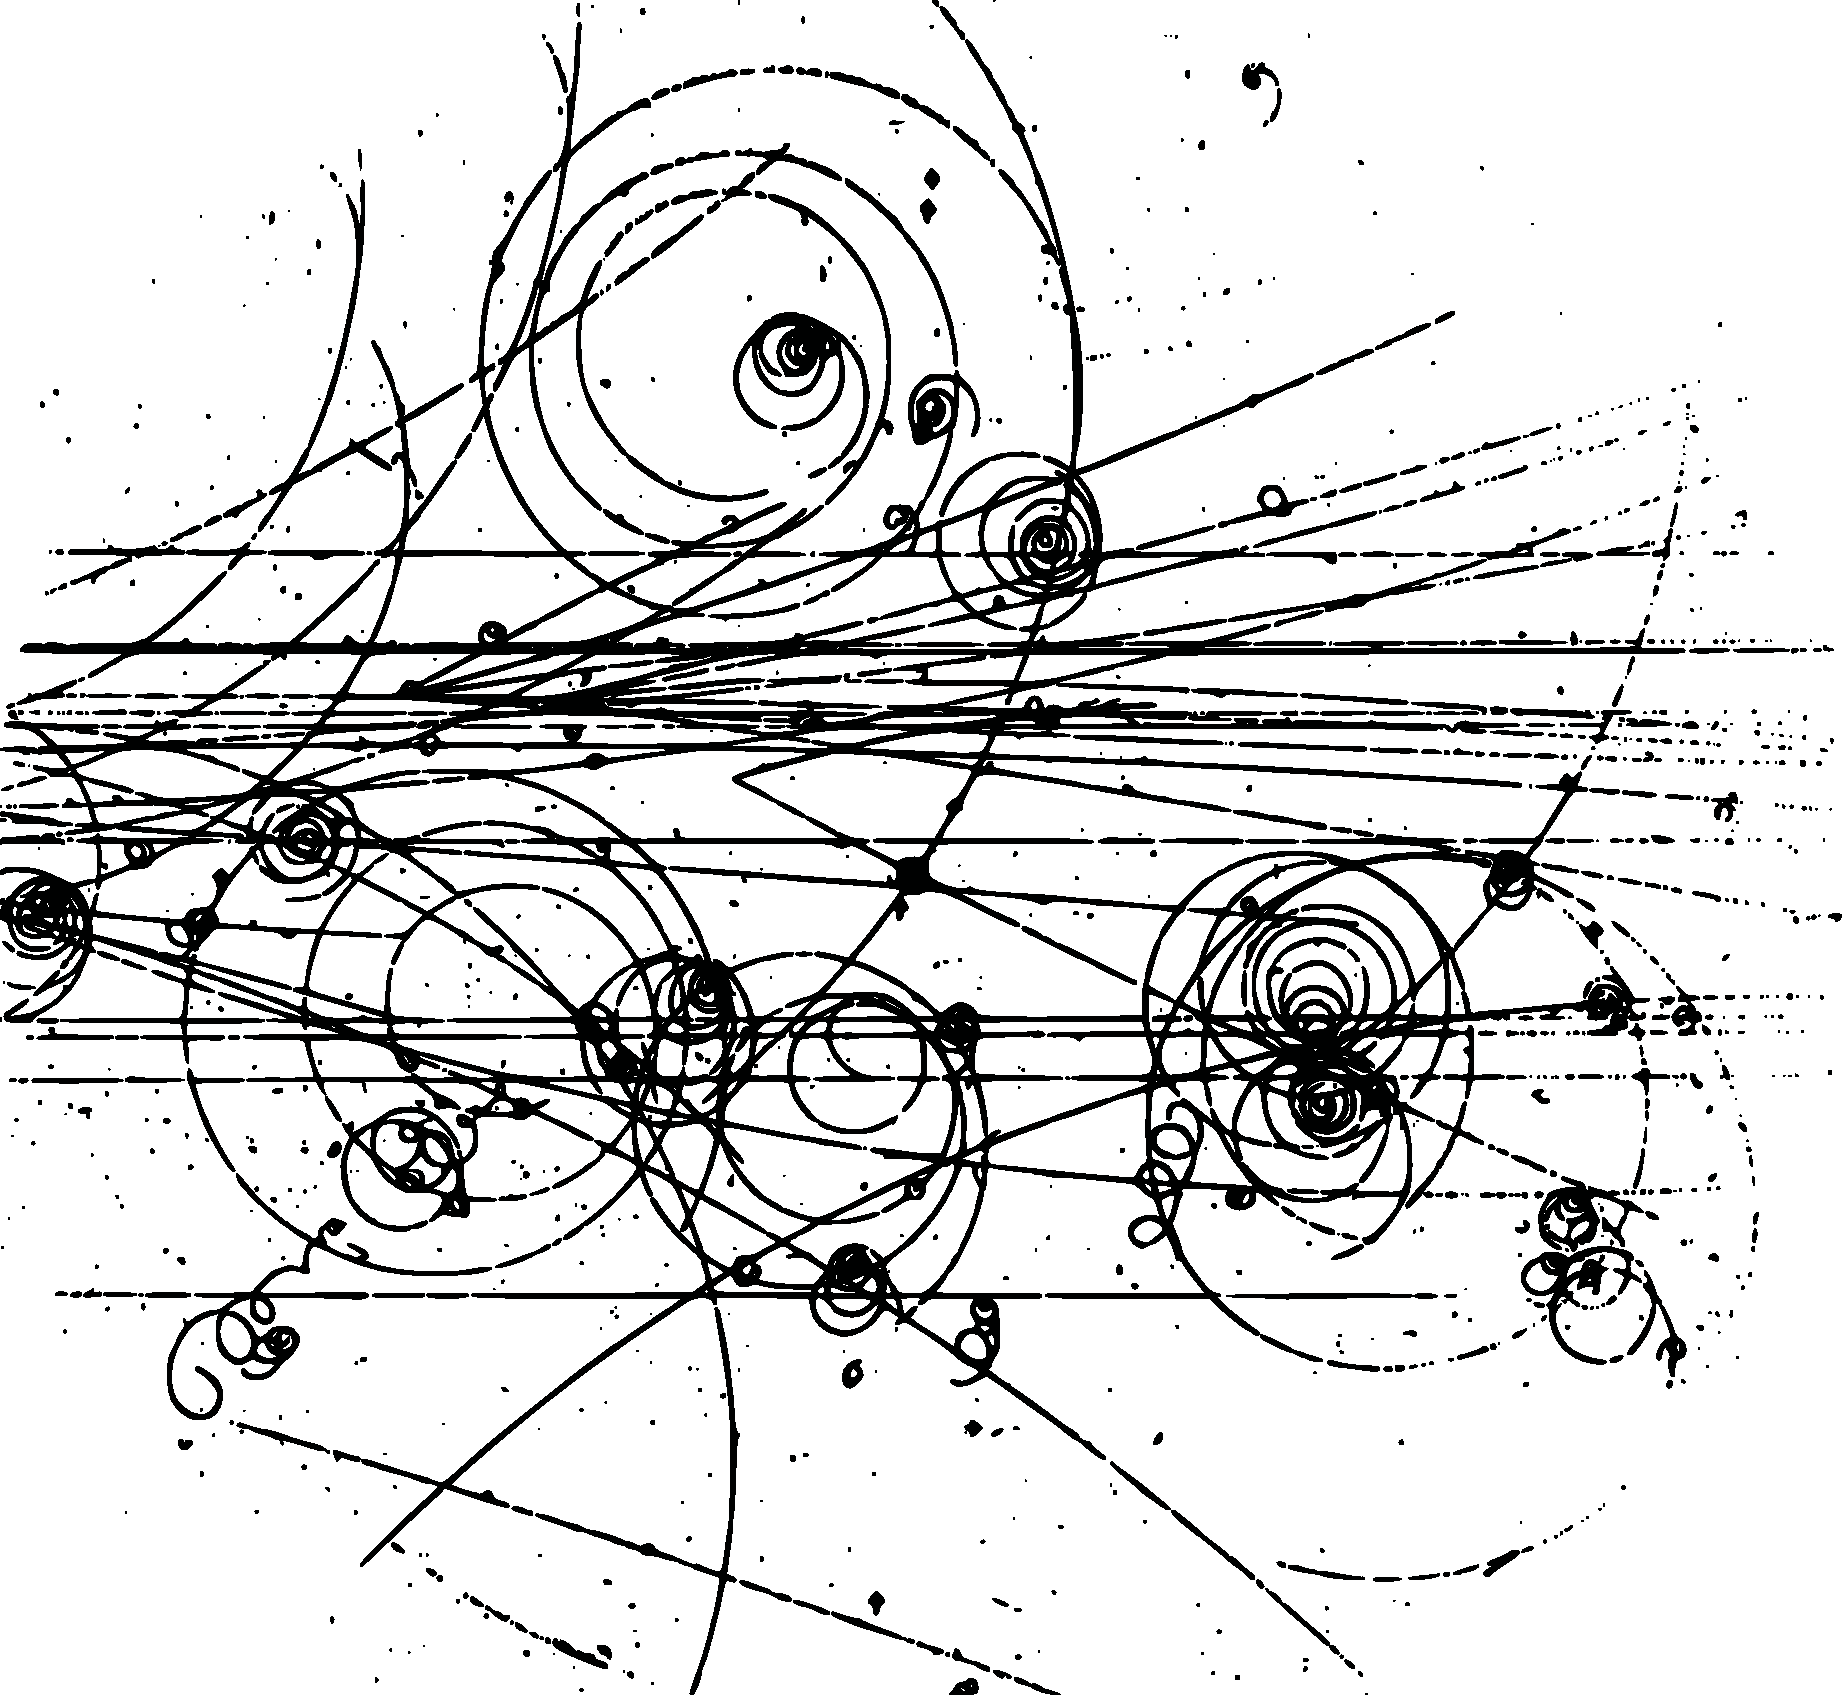
\includegraphics[width=0.6\linewidth]{fig/bc_1}}};
	\end{tikzpicture}
}

\newcommand\tocforsect[2]{%
	\begingroup
	\edef\safesection{\thesection}
	\setcounter{section}{#1}
	\tableofcontents[#2,currentsection]
	\setcounter{section}{\safesection}
	\endgroup
}

%----------------------------------------------------------------------------------------

\begin{frame}[t]{Overview}
\only<1>{\tocforsect{1}{sectionstyle=shaded,subsectionstyle=shaded}}
\end{frame}

%----------------------------------------------------------------------------------------
\section{Introduction} 
%----------------------------------------------------------------------------------------

\begin{frame}[t]
\frametitle{Introduction I -- Standard Model}
\small
\vspace{-3mm}
\begin{block}{}
	\begin{itemize}
		\item The Standard Model (SM) is a basic theory which describes elementary particles and interactions between them
		\item Quarks: can be grouped into baryons ($q_1q_2q_3$) or mesons ($\bar q_1 q_2$)
		\item Focus of this analysis are $B$ mesons: $B^+(\bar b u)$ and $B^-(b \bar u)$
	\end{itemize}
\end{block}

\begin{center}
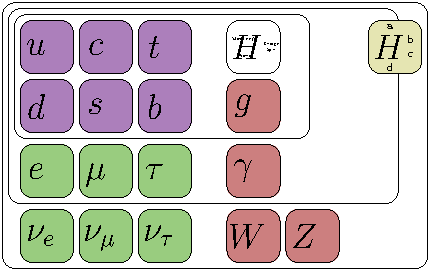
\includegraphics[scale=0.9]{texfig/SM}
\end{center}
\end{frame}

%----------------------------------------------------------------------------------------

\begin{frame}[t]
\frametitle{Introduction II -- $CP$ Violation}
\small
\vspace{-4mm}
\begin{block}{}
	\begin{itemize}
		\item {\color{blue}$C$} (charge conjugation), {\color{blue}$P$} (parity) and {\color{blue}$T$} (time reversal) symmetries were believed to be conserved individually (based on EM interaction, 1954)
		\item Observation of {\color{blue}$P$} symmetry violation confused physicists (1956)
		\item Observation of {\color{blue}$CP$} symmetry violation confused physicists even more (1964)
	\end{itemize}
\end{block}

$CP$ symmetry? $\to$ A sort of a "physics mirror", stating that the laws of physics should be the same if observed through said mirror.

\vspace{-2mm}
\begin{columns}
	\column{0.27\textwidth}
	\column{0.43\textwidth}
	\begin{block}{}
	\begin{itemize}
		\item $CP$ violation one of the necessary conditions for matter and antimatter asymmetry in the universe
		\item This analysis is one of the many steps toward a better understanding of our universe
	\end{itemize}
	\end{block}
	\column{0.3\textwidth}
\end{columns}

\begin{picture}(0,0)
\put(0,5){
	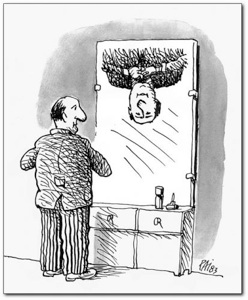
\includegraphics[scale=0.35]{fig/cpv}}
\end{picture}

\begin{picture}(0,0)
\put(0,6){
	{\tiny\texttt{\url{http://pprc.qmul.ac.uk/~still/homepage/Matter_and_Anti-Matter.html}}}
}
\end{picture}

\begin{picture}(0,0)
\put(250,30){
	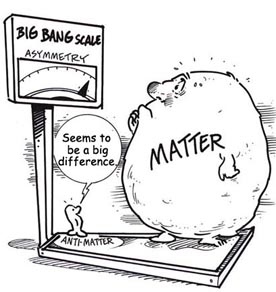
\includegraphics[scale=0.35]{fig/asymmetry}}
\end{picture}


\end{frame}

%----------------------------------------------------------------------------------------

\begin{frame}[t]
\frametitle{Introduction III -- CKM Matrix}
\small
\vspace{-3mm}
\begin{block}{}
	\begin{itemize}
		\item $CP$ violation is described by the Cabibbo-Kobayashi-Maskawa (CKM) matrix
		\item It is a complex and unitary matrix
		\item Contains transition probabilities from one quark to the other (charged weak interaction)

	\end{itemize}
	$$V_{CKM} = \begin{bmatrix} V_{ud} & V_{us} & V_{ub} \\ V_{cd} & V_{cs} & V_{cb} \\ V_{td} & V_{ts} & V_{tb} \end{bmatrix}, \quad \vert V_{ij}\vert^2 \propto q_i \leftrightarrow q_j~~\mathrm{transition~probability} $$
\end{block}

\begin{center}
	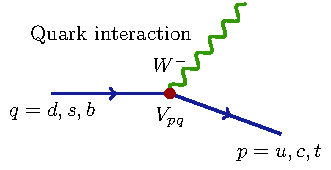
\includegraphics[scale=0.95]{texfig/quark_transition}
	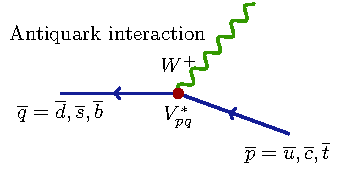
\includegraphics[scale=0.95]{texfig/antiquark_transition}
\end{center}

\end{frame}

%----------------------------------------------------------------------------------------

\begin{frame}[t]
\frametitle{Introduction IV -- Unitarity Triangle}
\small
\vspace{-3mm}
\begin{block}{}
	\begin{itemize}
		\item The most relevant unitarity condition of the CKM matrix for this analysis is
		$$V_{ud}V_{ub}^{*}+V_{cd}V_{cb}^{*}+V_{td}V_{tb}^{*} = 0$$
	\end{itemize}
\end{block}

\begin{center}
	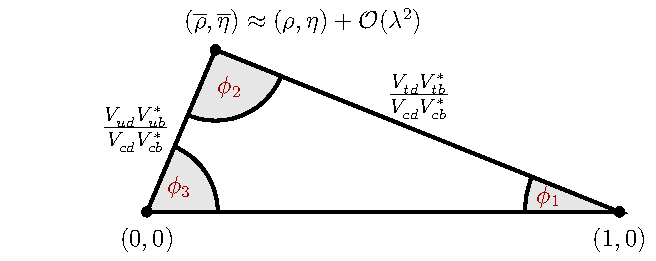
\includegraphics[scale=0.8]{texfig/UT_Triangle}
\end{center}
\vspace{-2mm}
\begin{block}{}
\begin{itemize}
	\item By measuring the sides and angles of the triangle, we can overconstrain it and check if all the sides meet
	\item CKM matrix elements are not determined by theory or experiment alone, but by their joint effort
\end{itemize}
\end{block}

\end{frame}

%----------------------------------------------------------------------------------------

\begin{frame}[t]
\frametitle{Introduction V -- Unitarity Triangle Determination}
\small
\vspace{-3mm}
\begin{block}{}
	\begin{itemize}
		\item The most relevant unitarity condition of the CKM matrix for this analysis is
		$$V_{ud}V_{ub}^{*}+V_{cd}V_{cb}^{*}+V_{td}V_{tb}^{*} = 0$$
	\end{itemize}
\end{block}
\vspace{-2mm}

\begin{center}
		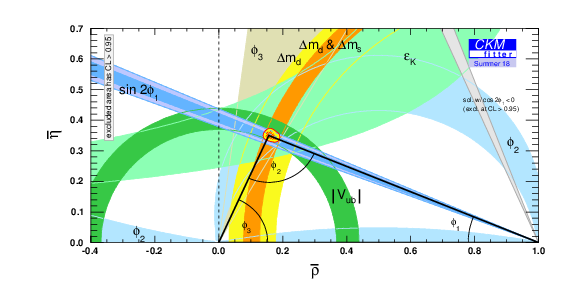
\includegraphics[width=0.9\textwidth]{fig/belle_rhoeta_small_global}
\end{center}

\vspace{-2mm}

In this analysis we focus on decays involving $\textcolor{red}{V_{ub}}$

\end{frame}

%----------------------------------------------------------------------------------------
\section{Motivation} 
%----------------------------------------------------------------------------------------

\begin{frame}[t]{Overview}
\only<1>{\tocforsect{2}{sectionstyle=shaded,subsectionstyle=shaded}}
\end{frame}

%----------------------------------------------------------------------------------------

\begin{frame}[t]{Motivation I -- Why $V_{ub}$?}
\small
\vspace{-3mm}
\begin{block}{}
	\begin{itemize}
		\item The magnitude of $CP$ violation that we know of is not large enough to account for the matter and antimatter asymmetry
		\item We are searching for new physics (NP) processes, which are not described by our current model
		\item \textcolor{red}{$\vert V_{ub}\vert$} has the smallest value and the largest uncertainty of all the CKM matrix elements, precision measurements require better accuracy
	\end{itemize}
\end{block}

\begin{center}
	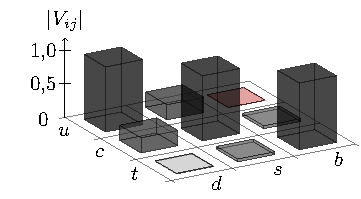
\includegraphics[width=0.6\textwidth]{texfig/fig_CKM}
\end{center}


%{
%	\large
%	$$V_{CKM} = \begin{bmatrix} V_{ud} & V_{us} & \textcolor{red}{V_{ub}} \\ V_{cd} & V_{cs} & V_{cb} \\ V_{td} & V_{ts} & V_{tb} \end{bmatrix}$$
%}
%- why B mesons
%- why Vub
%- Vub determination
%- analysis decay
\end{frame}


%----------------------------------------------------------------------------------------

\begin{frame}[t]{Motivation II -- Why $B$ Mesons?}
\small
\vspace{-3mm}
\begin{block}{}
	\begin{itemize}
		\item $B$ mesons exhibit a rich spectrum of decay modes, out of which many allow the study of the underlying physics processes
		\item Decays are deeply connected to the CKM matrix
	\end{itemize}
\end{block}

\begin{exampleblock}{}
	\begin{itemize}
		\item We focus on the charmless semileptonic $B$ meson decays of the form $B^+ \to X_u^0 \ell^+ \nu_\ell$ (inclusion of charge conjugated $B^-$ decays is implied)
		\item Such decays are used to determine the $\vert V_{ub}\vert$ CKM matrix element
	\end{itemize}
\end{exampleblock}

\begin{columns}
	\column{0.45\textwidth}
	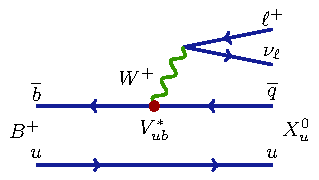
\includegraphics[scale=1]{texfig/B2pilnu_short}
	\column{0.55\textwidth}
	Reliable \textcolor{turtlegreen}{experimental measurements} along with precise \textcolor{blue}{theoretical calculations} enable the determination of the \textcolor{red}{$\vert  V_{ub} \vert$}
	\begin{equation*}
	\textcolor{turtlegreen}{\mathrm{d} \Gamma} \propto G_F^2 \vert \textcolor{red}{ V_{ub}} \vert ^2 \vert \textcolor{blue}{L^\mu \langle X_u \vert \bar u \gamma_\mu \frac{1}{2} (1-\gamma_5) b \vert B \rangle} \vert ^2,
	\end{equation*}
	
$\Gamma$ is the decay width, $L^\mu$ is the leptonic current and $\langle \dots \rangle$ is the hadronic current.
\end{columns}
\end{frame}

%----------------------------------------------------------------------------------------

\begin{frame}[t]{Motivation III -- Why This Analysis?}
\small
\vspace{-3mm}
There are two common methods of $\vert V_{ub}\vert $ determination
\begin{columns}
	\column{0.49\textwidth}
	\begin{block}{}
		Exclusive
		\begin{itemize}
			\item $B$ decays to a specific hadronic final state $X_u$ (such as $\pi$ or $\rho$)
		\end{itemize}
\begin{center}
	\vspace{-3mm}
		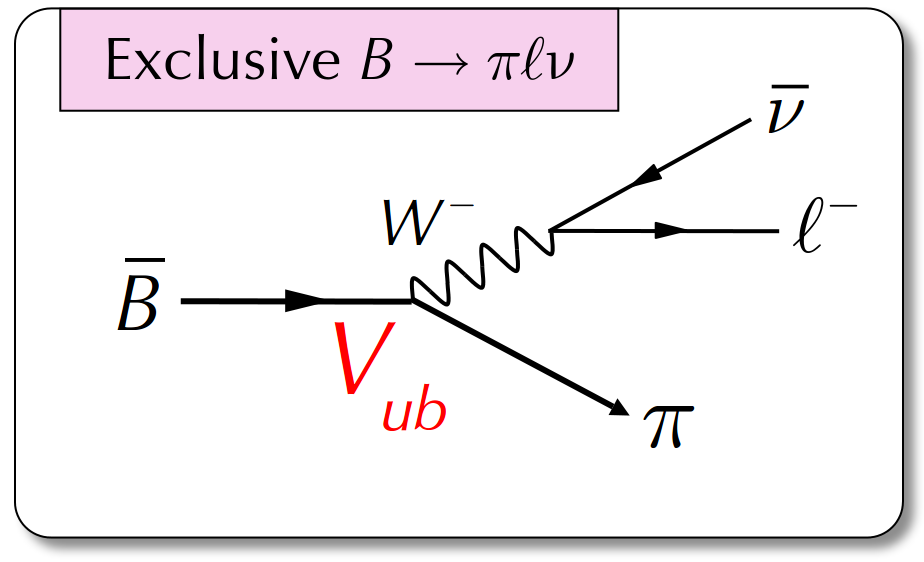
\includegraphics[width=0.5\textwidth]{fig/excl}
\end{center}
	\end{block}
	\column{0.49\textwidth}
	\begin{block}{}
		Inclusive
		\begin{itemize}
			\item $B$ meson decays to any hadronic final state $X_u$
		\end{itemize}
\begin{center}
	\vspace{-3mm}
	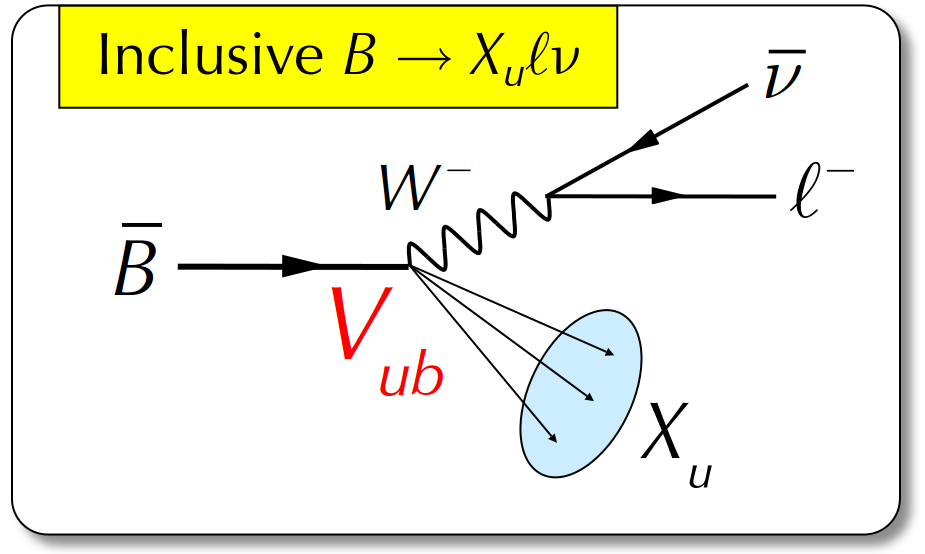
\includegraphics[width=0.5\textwidth]{fig/incl}
\end{center}
\end{block}
\end{columns}

\vspace{3mm}
Both methods require different experimental and theoretical approaches, therefore yield largely independent results
\begin{align*}
&\vert V_{ub} \vert_{\mathrm{excl.}} = \left(3.65 \pm 0.09 \pm 0.11\right)\E{-3},\\
&\vert V_{ub} \vert_{\mathrm{incl.}}^{\mathrm{GGOU}} = \left(4.52 \pm 0.15~{}^{+0.11}_{-0.14}\right)\E{-3},
\end{align*}
\textcolor{red}{However, they agree only at a $3\sigma$ level} $\to$ The $V_{ub}$ puzzle

\end{frame}

%----------------------------------------------------------------------------------------

\begin{frame}[t]{Motivation IV -- Why This Decay?}
\small
\vspace{-3mm}
\begin{block}{}
	\begin{itemize}
		\item Primary: The decay has not been observed yet
		\item The decay $B \rightarrow KK\ell\nu$ is similar to the $B \rightarrow \pi\ell\nu$ decay, so a similar analysis process can be applied
		\item Kaons ($K^+(u \bar s)$) are usually present in $b \to c (\to s)$ decays, so a $K$-veto is used to remove such background cases in inclusive $V_{ub}$ studies\\$\to$ \textcolor{red}{but this is a charmless process ($b \to u$) with kaons in the final state!}
		\item Secondary: Impact of not taking these decays into account?
	\end{itemize}
\end{block}

\begin{columns}
	\column{0.45\textwidth}
	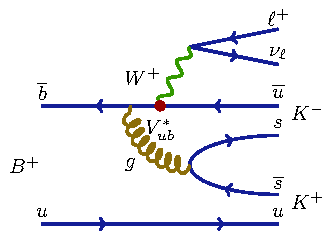
\includegraphics[scale=0.9]{texfig/B2KKlnu}
	\column{0.45\textwidth}
	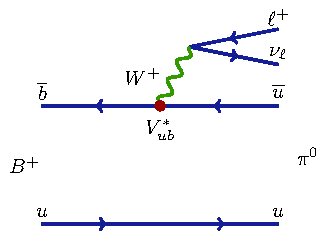
\includegraphics[scale=0.9]{texfig/B2pilnu}
\end{columns}


\end{frame}

%----------------------------------------------------------------------------------------
\section{Experimental Setup} 
%----------------------------------------------------------------------------------------

\begin{frame}[t]{Overview}
\only<1>{\tocforsect{3}{sectionstyle=shaded,subsectionstyle=shaded}}
\end{frame}

%----------------------------------------------------------------------------------------

\begin{frame}[t]
\frametitle{Experimental Setup I -- KEKB Accelerator}
\vspace{-3mm}
\small

\begin{columns}
	\column{0.6\textwidth}
	\begin{block}{}
		\begin{itemize}
			\item Two rings ($e^+$ and $e^-$) with a diameter $ \approx 1$ km
			\item Particles are produced in events when $e^+$ and $e^-$ collide
			\item Energy in the center-of-mass frame is 10.58 GeV
			\begin{itemize}
				\item corresponds to $\Upsilon(4S)$ meson mass
			\end{itemize}
			\item B factories are known for abundant production of $B$ mesons
		\end{itemize}
	\end{block}
	
	\column{0.4\textwidth}
	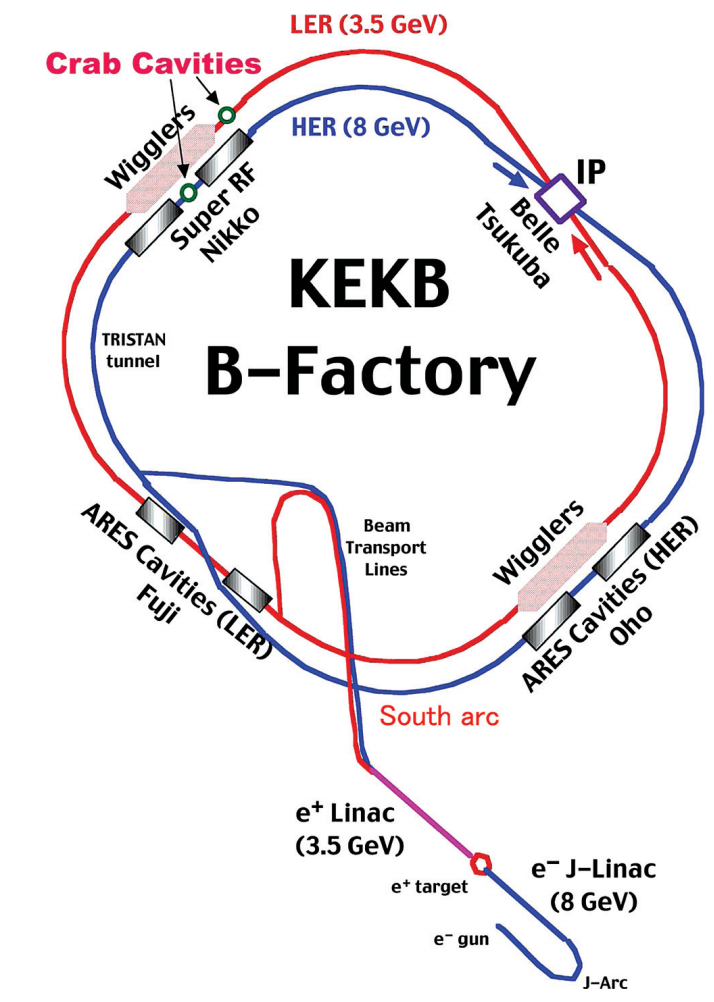
\includegraphics[scale=0.2]{fig/setup/KEKB}	
\end{columns}

\end{frame}

%----------------------------------------------------------------------------------------

\begin{frame}[t]
\frametitle{Experimental Setup II -- Particle Detection}
\vspace{-3mm}
\small

\only<1>{
		\begin{center}
		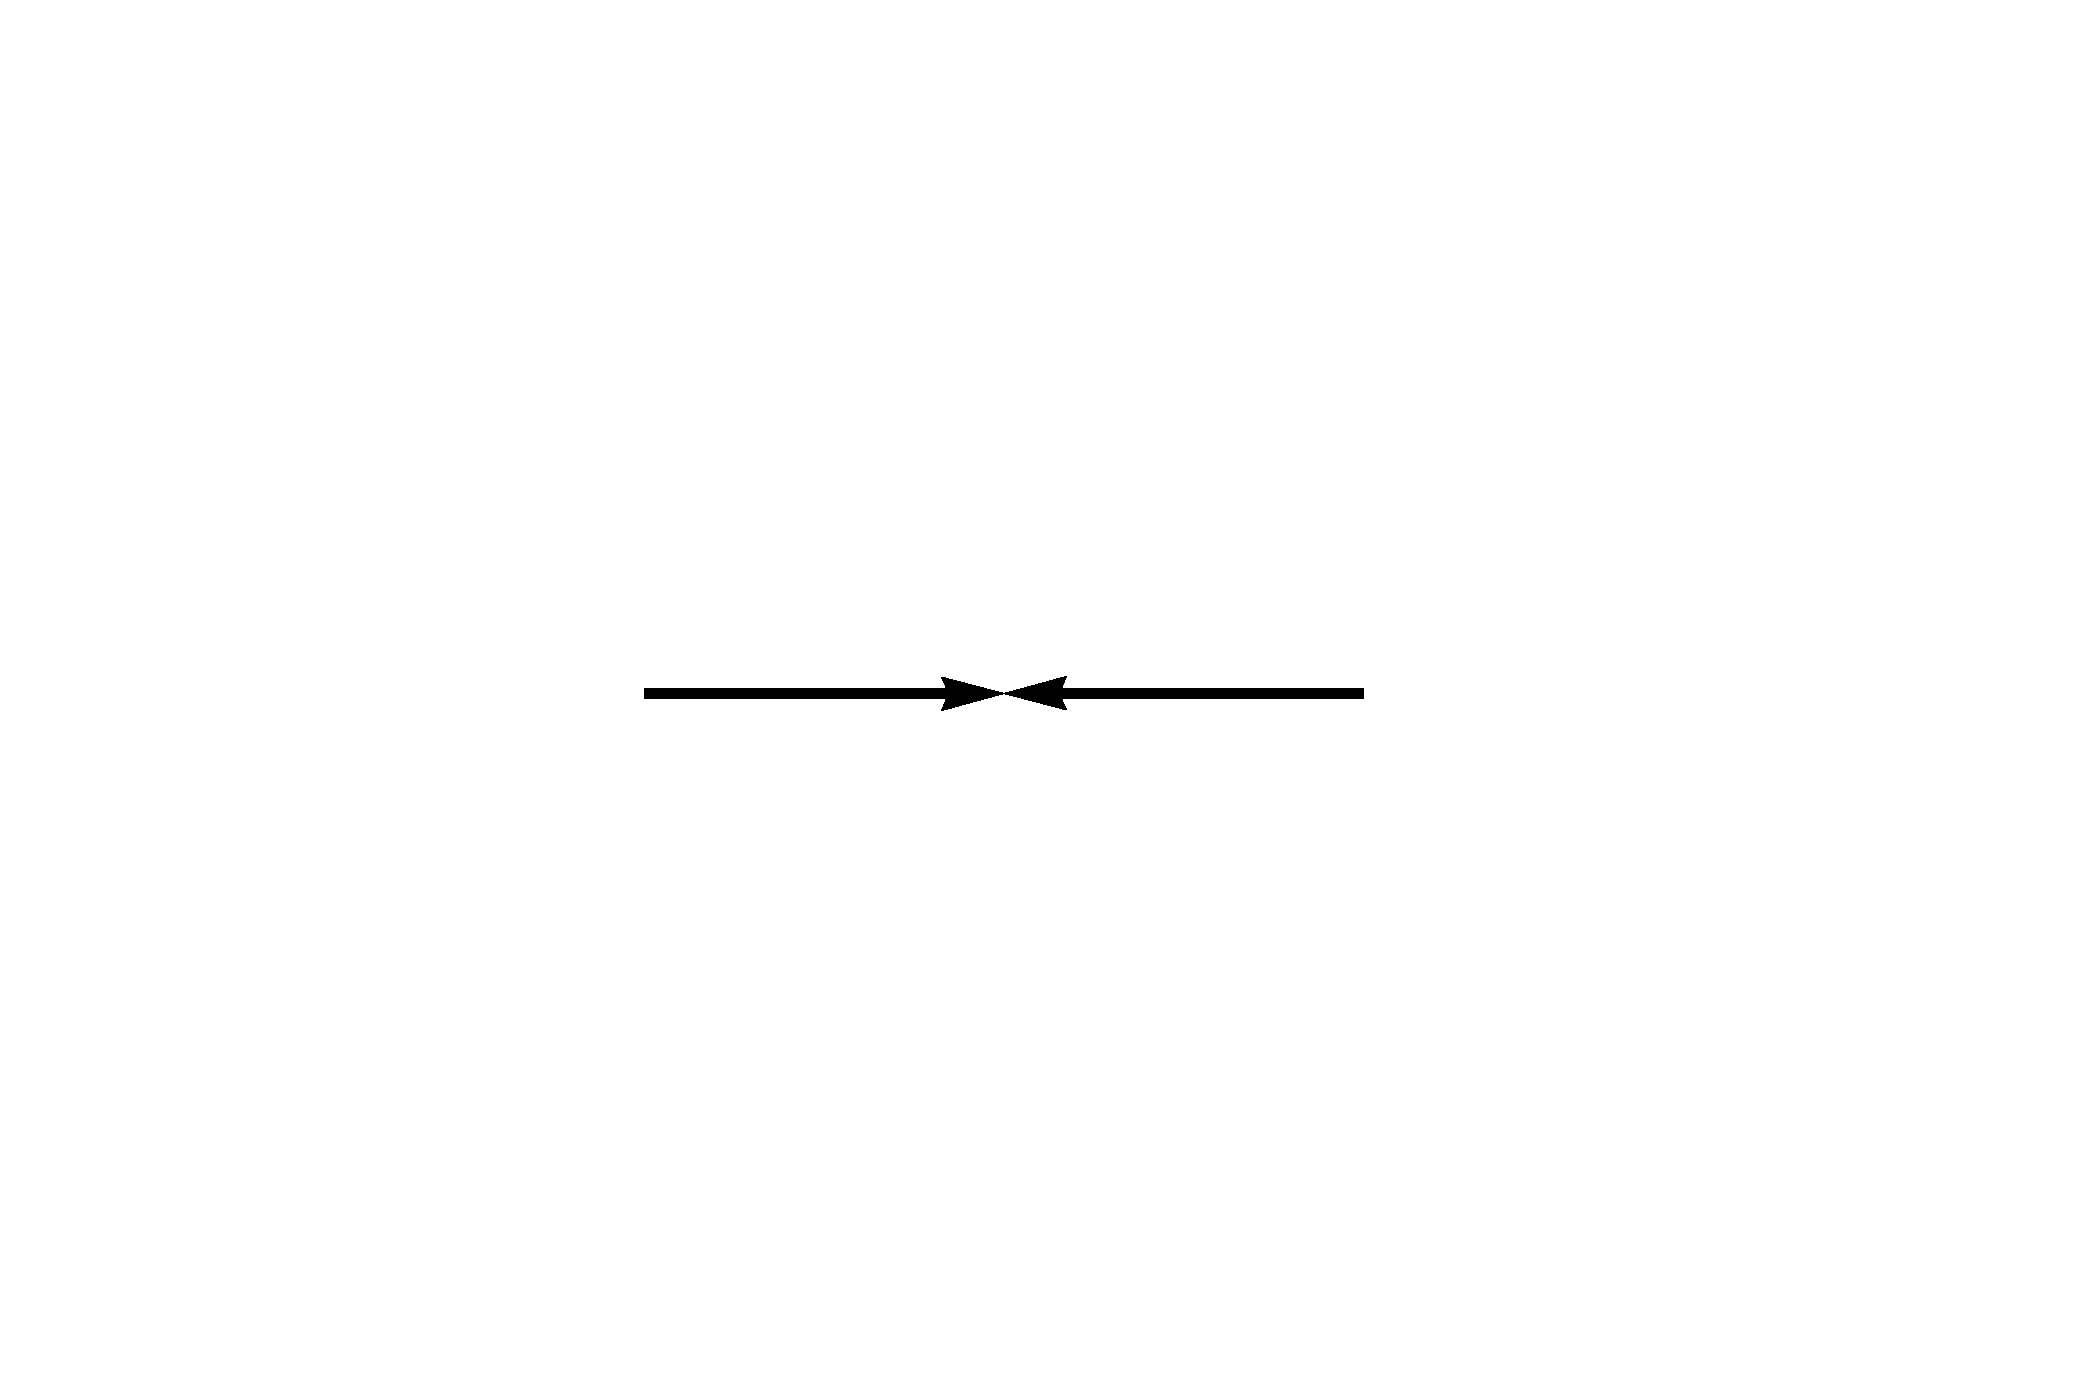
\includegraphics[width=0.6\textwidth]{fig/sim_1}
	\end{center}
	\begin{block}{}
	\begin{itemize}
		\item Event -- collision of $e^+$ and $e^-$
	\end{itemize}
\end{block}
}

\only<2>{
		\begin{center}
		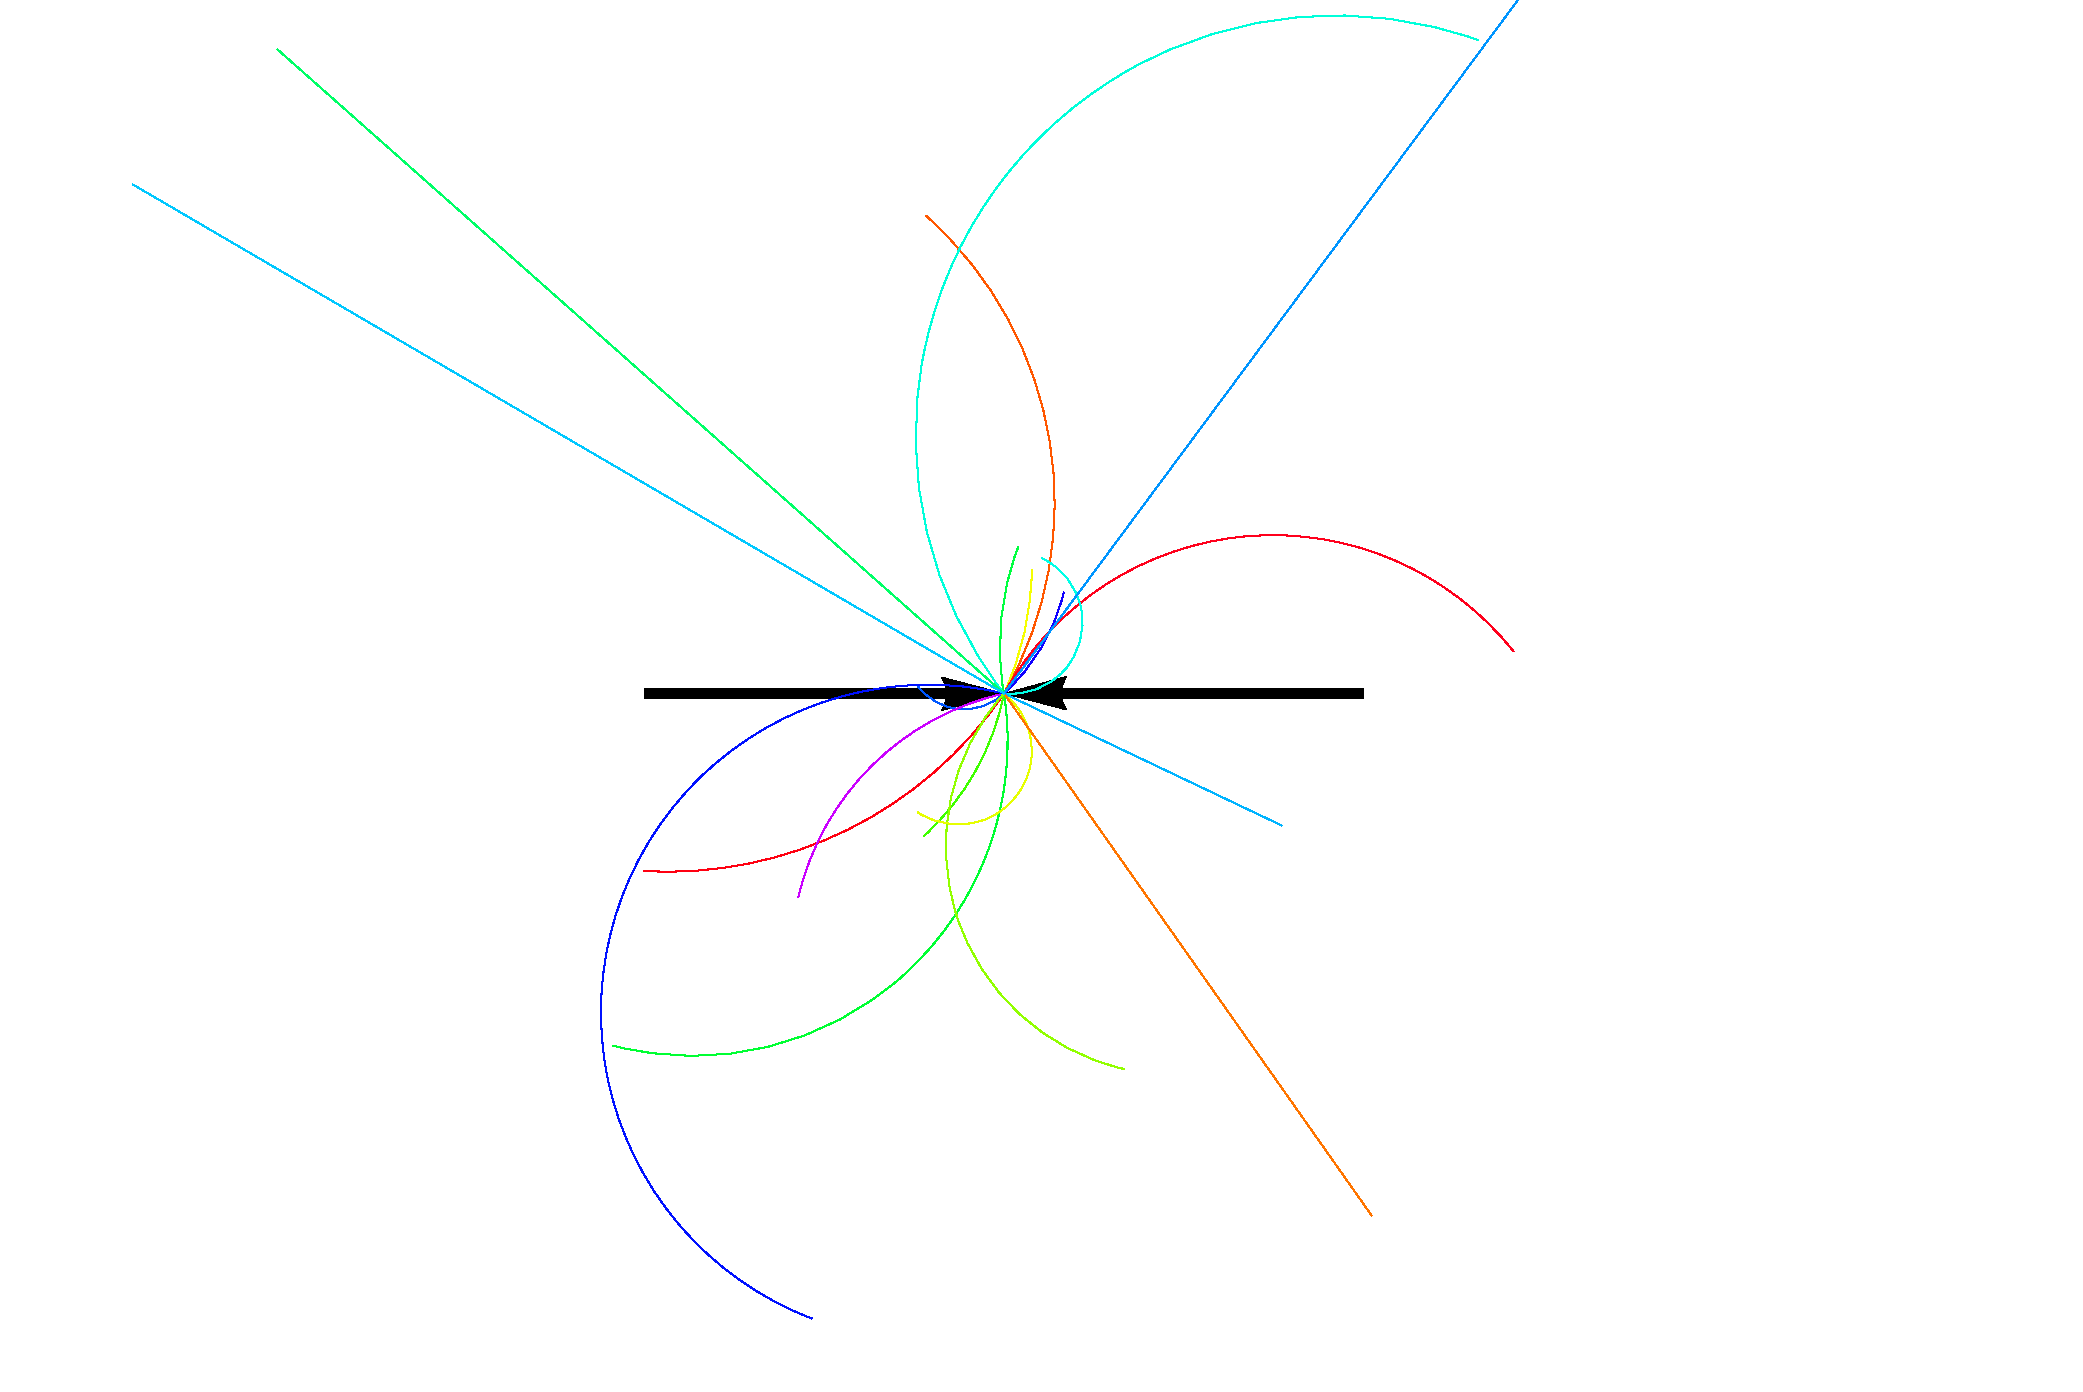
\includegraphics[width=0.6\textwidth]{fig/sim_2}
	\end{center}
		\begin{block}{}
		\begin{itemize}
			\item Event -- collision of $e^+$ and $e^-$
			\item Production of new particles
		\end{itemize}
	\end{block}
}

\only<3>{
		\begin{center}
		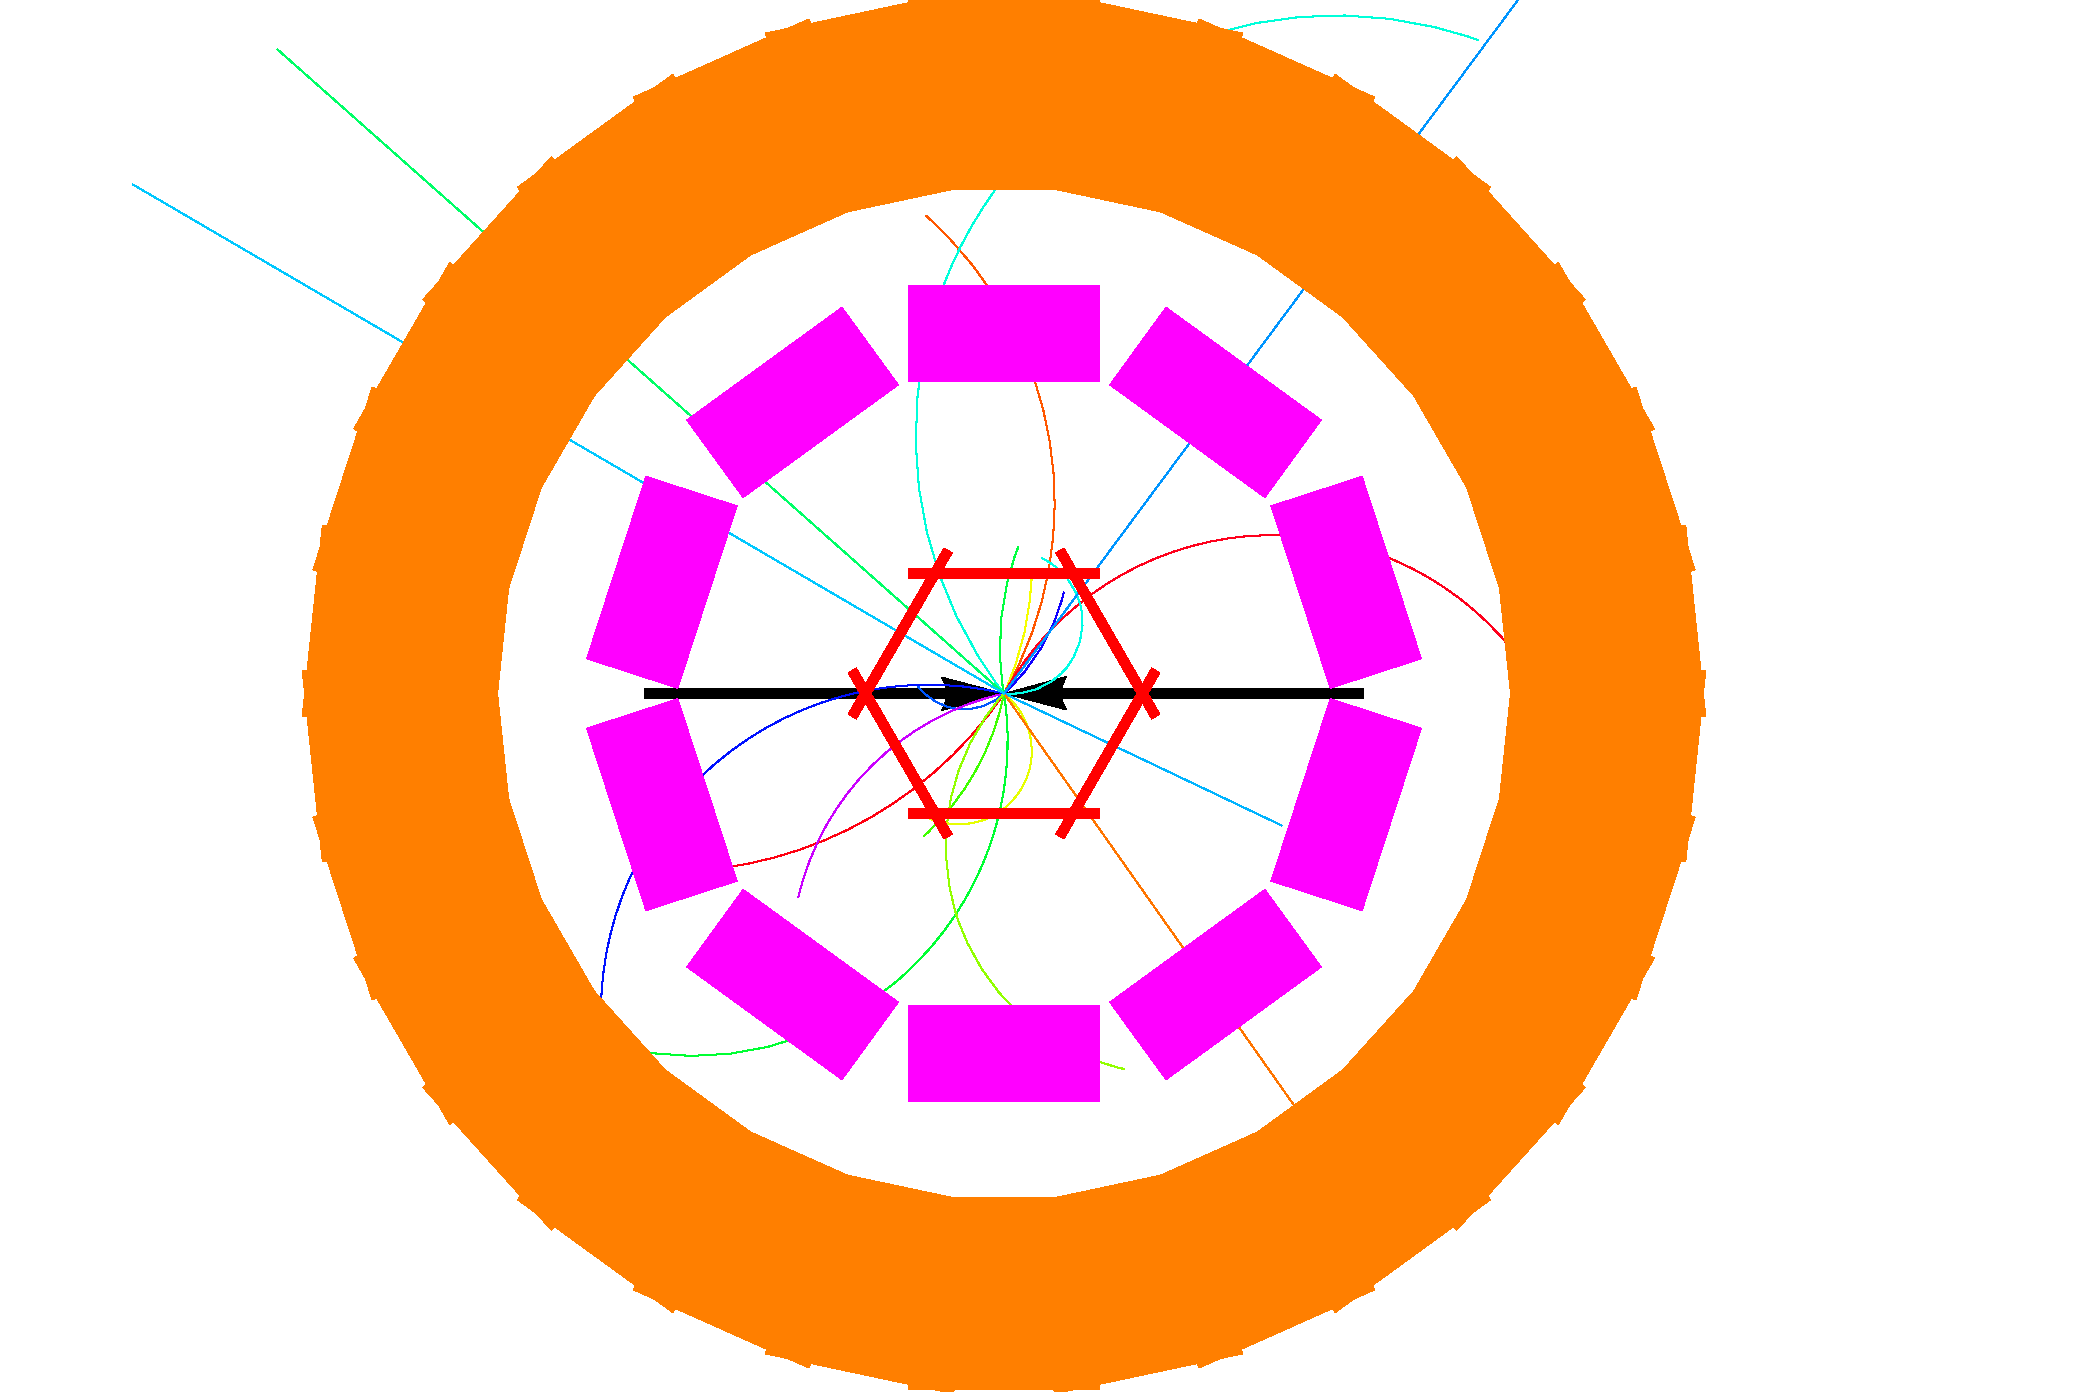
\includegraphics[width=0.6\textwidth]{fig/sim_3}
	\end{center}
		\begin{block}{}
		\begin{itemize}
			\item Event -- collision of $e^+$ and $e^-$
			\item Production of new particles
			\item Detection of final, stable particles
		\end{itemize}
	\end{block}
}

\end{frame}



%----------------------------------------------------------------------------------------

\begin{frame}[t]
\frametitle{Experimental Setup III -- Belle Detector}
\vspace{-3mm}
\small

\begin{block}{}
\begin{itemize}
\item A cylindrically symmetric magnetic spectrometer
\item Wide solid angle coverage ($\sim92\%$)
\item Specialized for $e^+e^-$ collisions
\item Constructed from several subdetectors, each with its own purpose
\end{itemize}
\end{block}

\begin{columns}
\column{0.5\textwidth}
Belle II detector subsystems:
\begin{itemize}
\item Decay vertex determination
\item Tracking
\item Particle identification
\item Calorimetry
\end{itemize}

\column{0.5\textwidth}
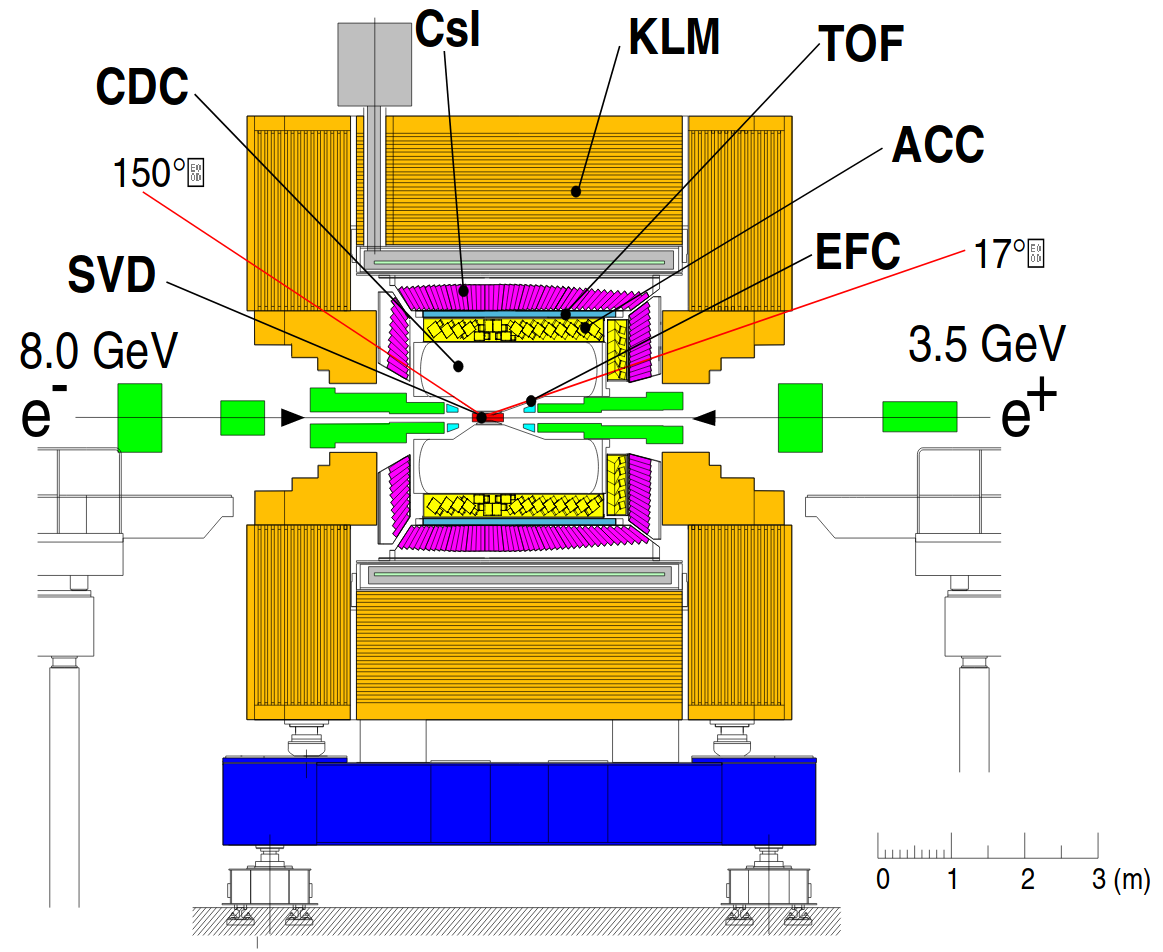
\includegraphics[scale=0.16]{fig/setup/Belle_detector}
\end{columns}

\end{frame}

%----------------------------------------------------------------------------------------

\begin{frame}[t]
\frametitle{Experimental Setup III -- Belle Detector Subsystems}
\vspace{-3mm}
\small

\begin{tikzpicture}
 \node {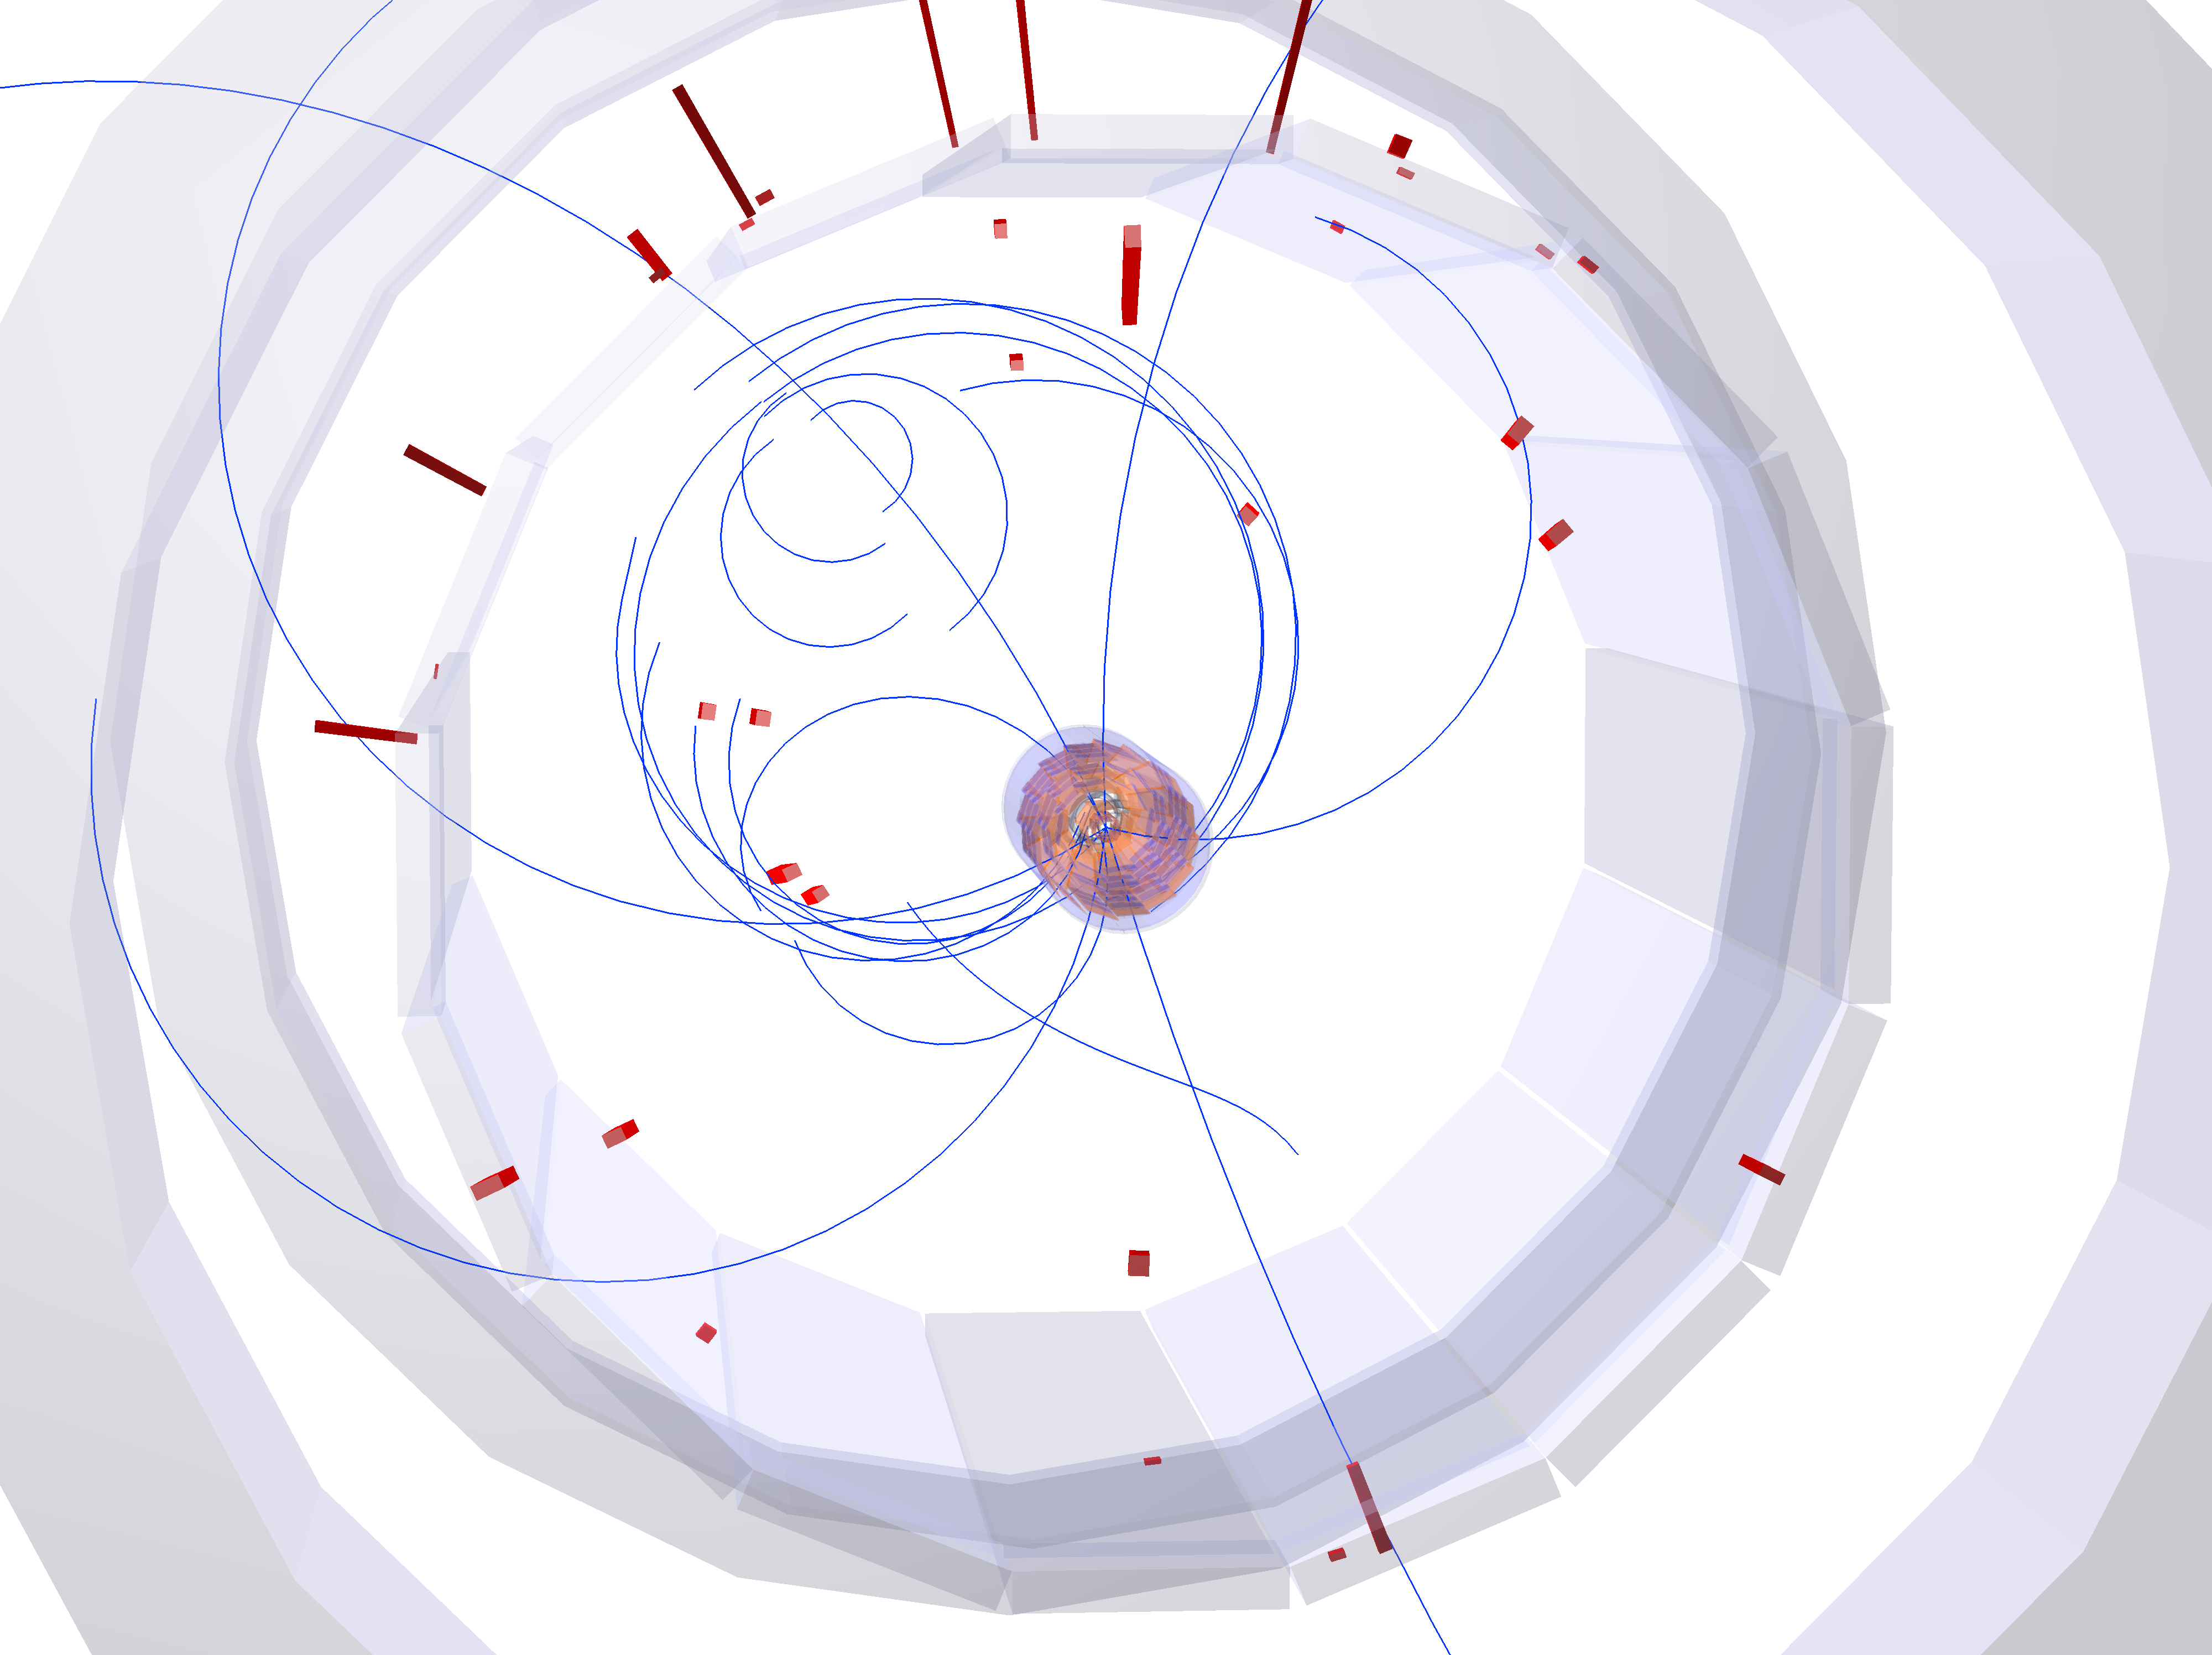
\includegraphics[width=\textwidth]{fig/display}};

 \node at (3.2,-3) {
 \begin{tabular}{l}
 Silicon Vertex Detector (SVD)\\
 Central Drift Chamber (CDC)\\
 Electromagnetic Calorimeter (ECL)\\
 \end{tabular}
};

\node at (4,3.5) {
	\begin{tabular}{l}
	\textcolor{turtlegreen}{Neutral Cluster}\\
	\textcolor{turtlegreen}{Charged Track}
	\end{tabular}
};

 \draw[thick, ->] (2.5,-2.3) to [out=90,in=0] (0.5,0);
 \draw[thick, ->] (0.3,-3.0) to [out=180,in=270] (-1.5,-1.5);
 \draw[thick, ->] (0.3,-3.4) to [out=180,in=270] (-3.8,0);
 
 \draw[thick, turtlegreen, ->] (4,3) to [out=-90,in=0] (2.2,1);
 \draw[thick, turtlegreen, ->] (2.6,3.7) to [out=180,in=0] (0.2,3);


\end{tikzpicture}

\end{frame}

%----------------------------------------------------------------------------------------

%----------------------------------------------------------------------------------------
\section{Analysis Procedure} 
%----------------------------------------------------------------------------------------

\begin{frame}[t]{Overview}
\only<1>{\tocforsect{4}{sectionstyle=shaded,subsectionstyle=shaded}}
\end{frame}

%----------------------------------------------------------------------------------------

\begin{frame}[t]
\frametitle{Analysis I -- Method overview}
\vspace{-3mm}
\small

\begin{itemize}
	\item Initial state well known: $e^+e^- \to \Upsilon(4S)$ @ $E_{CMS} \approx M_{\Upsilon(4S)}$
	\item $\Upsilon(4S)$ at rest $\to B \overline B$
	\item Kaons $K$ and the leptons $e$ and $\mu$ produce tracks $\to$ \textcolor{turtlegreen}{easily detectable}
	\item Neutrinos $\nu$ interact weakly and escape the detector $\to$ \textcolor{red}{missing energy and momentum}
%	\item Neutrino 4-momentum inferred from missing momentum in event (assuming only one neutrino missing)
\end{itemize}

\only<1>{
	\begin{tikzpicture}

\node (origin) at (0cm,0cm) {};
\node [left, text width=5cm,fill=blue!20,align=center] at (7cm,0cm){\large Reconstruction methods};
\node [left,text width=4.5cm,fill=green!20,align=center] at (3cm,-0.8cm){\large Tagged measurement};
\node [left,text width=5cm,fill=green!20,align=center] at (10cm,-0.8cm){\large Untagged measurement};
\node (img) at (1cm,-2.5cm) {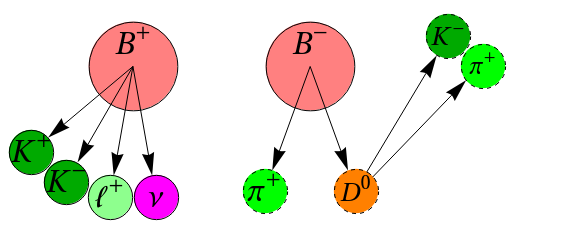
\includegraphics[scale=0.27]{fig/decay_5}};
\node (img) at (8cm,-2.5cm) {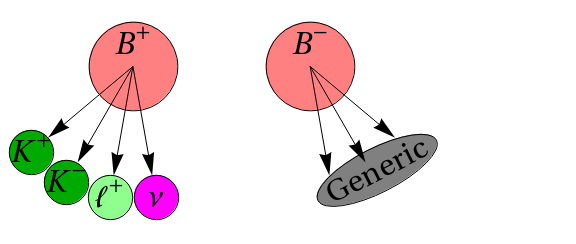
\includegraphics[scale=0.27]{fig/decay_3}};
\node [left,text width=5cm,fill=red!20,align=center] at (3.7cm,-4.3cm){\small Example scheme of a tagged mode};
\node [left,text width=5cm,fill=red!20,align=center] at (10cm,-4.3cm){\small Companion $B$ not reconstructed};

\end{tikzpicture}
}

\only<2>{
	\begin{tikzpicture}
	
	\node (origin) at (0cm,0cm) {};
	\node [left, text width=5cm,fill=blue!20,align=center] at (7cm,0cm){\large Reconstruction methods};
	\node [left,text width=5cm,fill=green!20,align=center] at (10cm,-0.8cm){\large Untagged measurement};
	\node (img) at (8cm,-2.5cm) {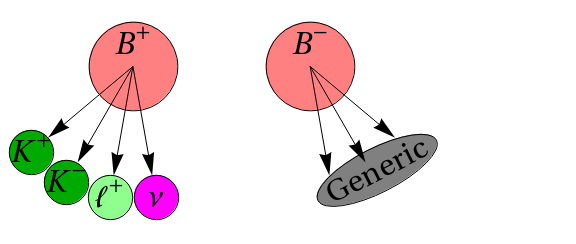
\includegraphics[scale=0.27]{fig/decay_3}};
	\node [left,text width=5cm,fill=red!20,align=center] at (10cm,-4.3cm){\small Companion $B$ not reconstructed};
	
	\node [left,text width=5cm,align=center] at (3.7cm,-2.5cm){
	\begin{tabular}{l}
	We opt for this method $\to$ \\
	Neutrino 4-momentum is inferred\\
	from missing momentum in event\\
	(assuming only 1 neutrino missing)
	\end{tabular}	
};
	
	\end{tikzpicture}
}

\end{frame}

%----------------------------------------------------------------------------------------

\begin{frame}[t]{Analysis II -- Particle Reconstruction}
%- particle reconstruction
%- ROE cleanup
%- loose neutrino reconstruction
%- control decay
%- final selection

\vspace{-3mm}
\small

\begin{block}{Part I: Final State Particles (FSP)}
\begin{itemize}
	\item Charged particles like $K$, $e$ and $\mu$ are reconstructed from tracks, a quality selection is performed
	\item Neutrinos are weakly interacting and escape detection
\end{itemize}
\end{block}

\begin{block}{Part II: FSP Combinations}
	\begin{itemize}
		\item Combinations of FSP particles $KKe$ and $KK\mu$ represent first $B$ meson candidates with a missing neutrino
	\end{itemize}
\end{block}

\begin{block}{Part III: Loose Neutrino Reconstruction}
	\begin{itemize}
		\item Rest of Event (ROE) are all the tracks (charged particles) and clusters (neutral particles) which were not used in the reconstruction
		\item ROE is needed to reconstruct the missing neutrino momentum, where all tracks and clusters from ROE are summed up together
	\end{itemize}
\end{block}


\end{frame}

%----------------------------------------------------------------------------------------

\begin{frame}[t]{Analysis III -- $B$ meson specific variables}

\vspace{-3mm}
\small

$$\Delta E = E_B - E_{CMS}/2,\quad M_{BC} = \sqrt{\left(E_{CMS}/2\right)^2 - \vert \vec{p}_B \vert^2}$$

\begin{center}
	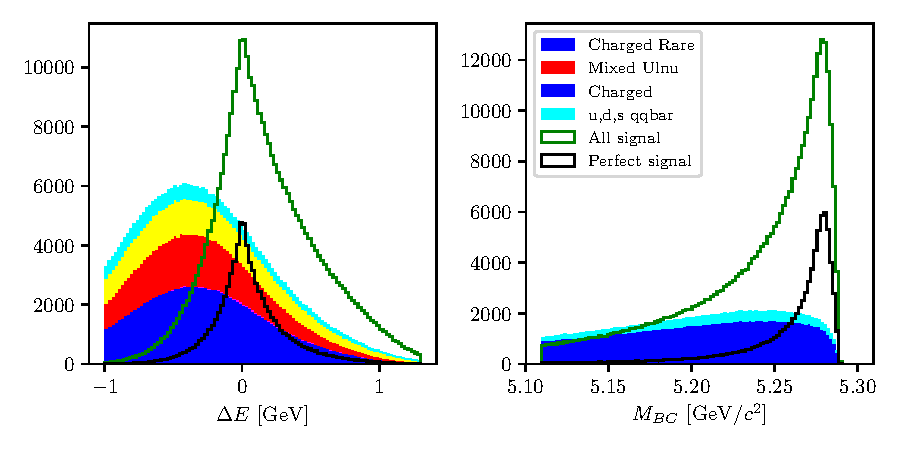
\includegraphics[width=0.98\textwidth]{fig/mbc_de_pre}
\end{center}

Signal is scaled up. Correctly reconstructed candidates have $\Delta E \approx 0$ and $M_{BC} \approx m_B$

\end{frame}


%----------------------------------------------------------------------------------------

\begin{frame}[t]{Analysis IV -- Control Decay}

\vspace{-3mm}
\small

\begin{block}{}
	We define a control decay mode, similar to our signal decay mode.
	\begin{itemize}
		\item The decay mode is $B^+ \to \bar D {}^0 \ell^+ \nu,\, D^0 \to K^+ K^-$
		\item The properties of the control and signal decay are very similar
		\item Its purpose is to continuously check the consistency between simulation (Monte Carlo or MC) and measured data
	\end{itemize}
\end{block}

\begin{center}
	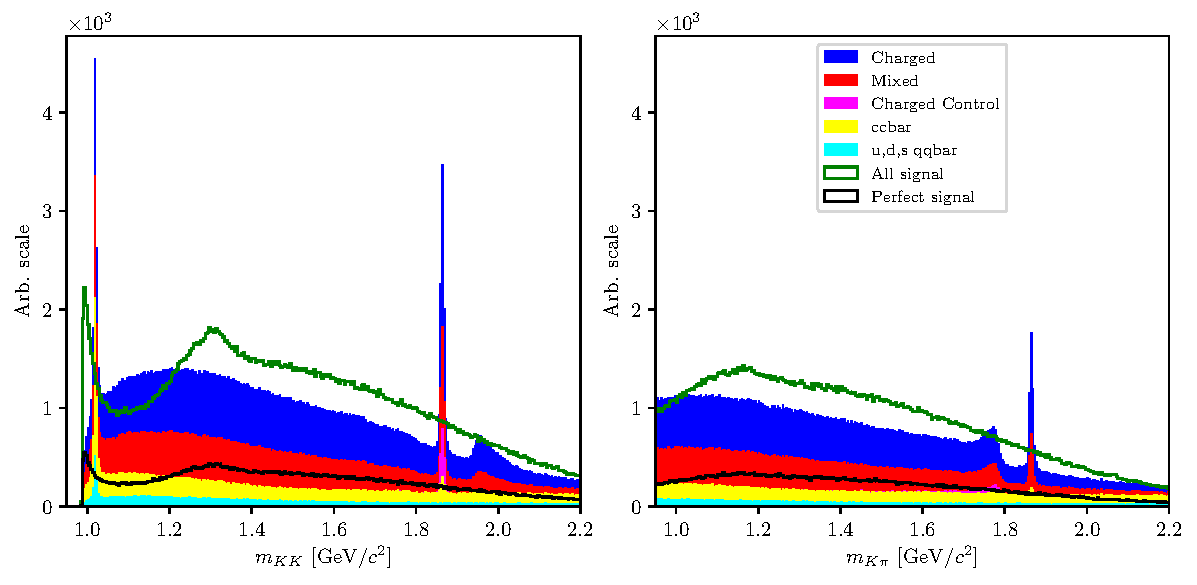
\includegraphics[width=\textwidth, trim={0 6.5cm 0 0},clip]{fig/res_bkg}
\end{center}

\end{frame}


%----------------------------------------------------------------------------------------


\begin{frame}[t]{Analysis V -- ROE Clean-up}
\vspace{-3mm}
\small

\begin{itemize}
	\item Rest of Event (ROE) are all the tracks (charged particles) and clusters (neutral particles) which were not used in the reconstruction
	\item ROE is needed to reconstruct the missing neutrino momentum
\end{itemize}
\begin{center}
	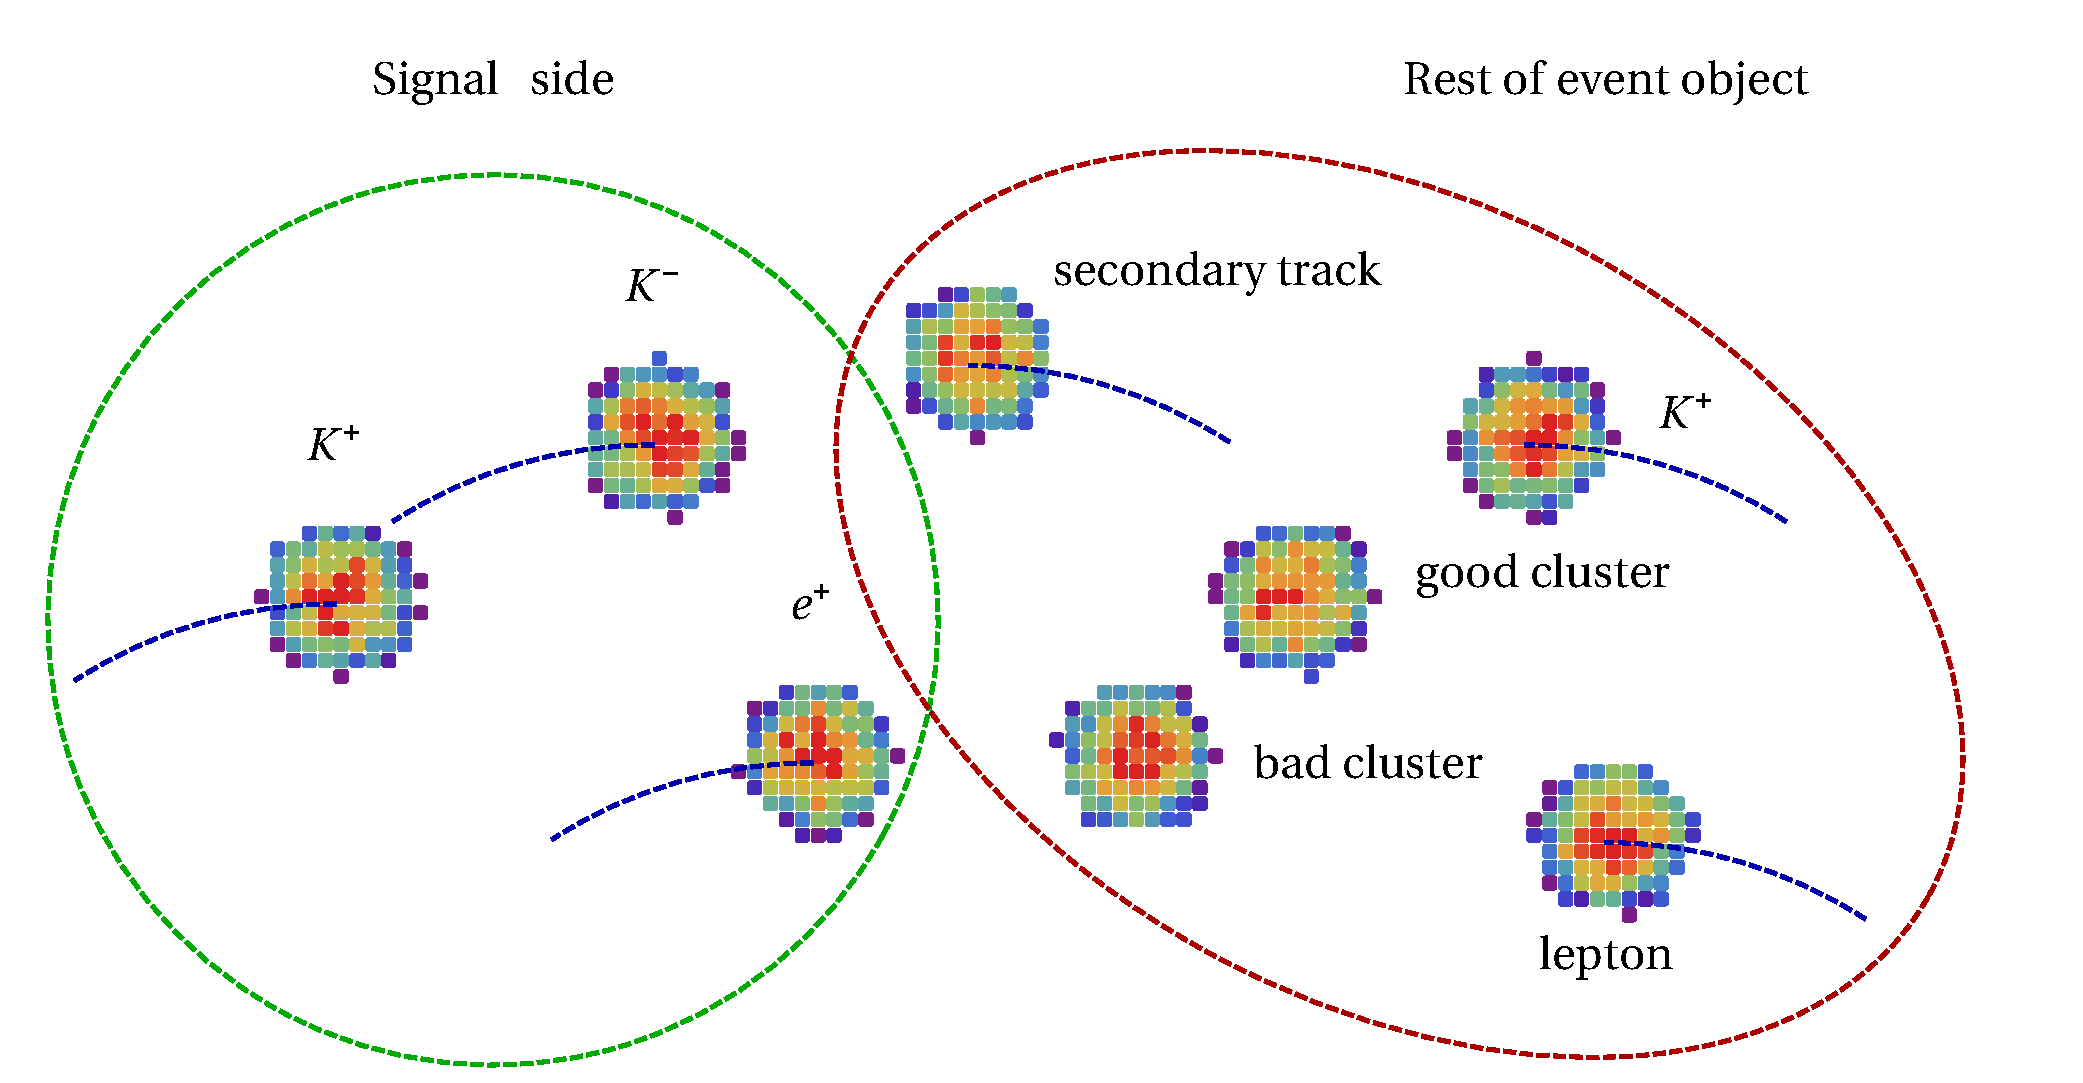
\includegraphics[width=0.6\textwidth]{fig/recon_5}
\end{center}

\vspace{-2mm}
\begin{block}{}
\begin{itemize}
	\item Why? Extra tracks and clusters should not be taken into account when calculating the neutrino 4-momentum
	\item How? We apply machine learning in several steps of the ROE clean-up in order to efficiently clean it
\end{itemize}
\end{block}

\end{frame}

%----------------------------------------------------------------------------------------

\begin{frame}[t]{Analysis VI -- ROE Clean-up Results}
\vspace{-3mm}
\small

\begin{columns}
	\column{0.6\textwidth}
	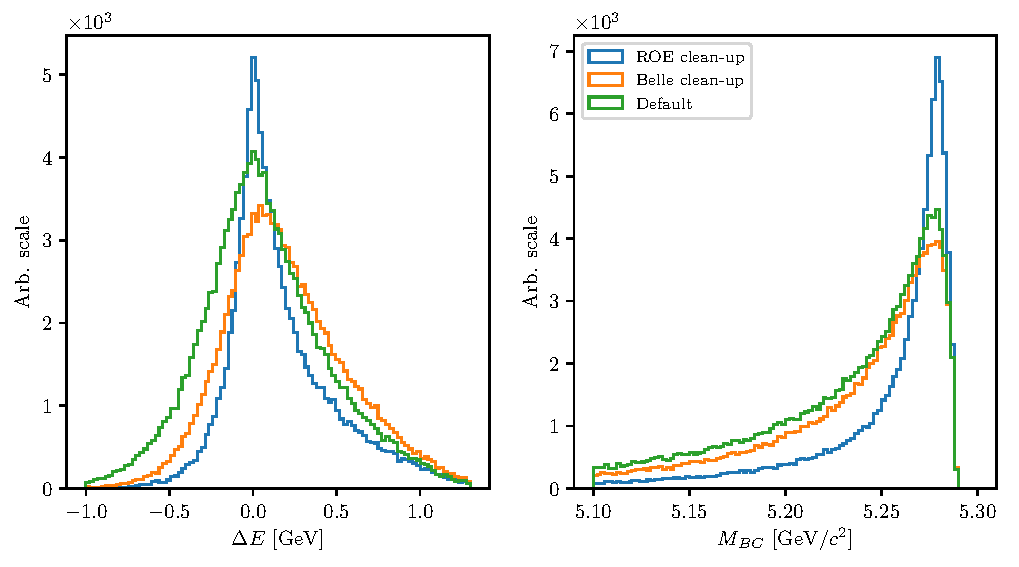
\includegraphics[width=\textwidth]{fig/roe_opt}
	\column{0.4\textwidth}
	\begin{block}{}
		\begin{itemize}
			\item The procedure \textbf{improves} \textbf{the resolution} of signal distribution
			\item It performs \textbf{better} than the standard Belle procedure
			\item \textbf{The efficiency} of perfectly reconstructed signal \textbf{increases}
		\end{itemize}
	\end{block}
	\begin{table}[H]
		\centering
		\begin{tabular}{c|c|c}
			& $\mathcal{E}$ & FWHM\\
			\toprule
			Belle & $28.5~\%$  & $75.0~\%$  \\
			ROE & $140.1~\%$ & $35.0~\%$ \\
			\bottomrule
		\end{tabular}
	\end{table}
\end{columns}

{\footnotesize Perfectly reconstructed signal candidates are signal candidates from events, where all tracks and clusters are accounted for.}


\end{frame}

%----------------------------------------------------------------------------------------

\begin{frame}[t]{Analysis VI -- ROE Clean-up Results}
\vspace{-3mm}
\small

\begin{columns}
	\column{0.6\textwidth}
	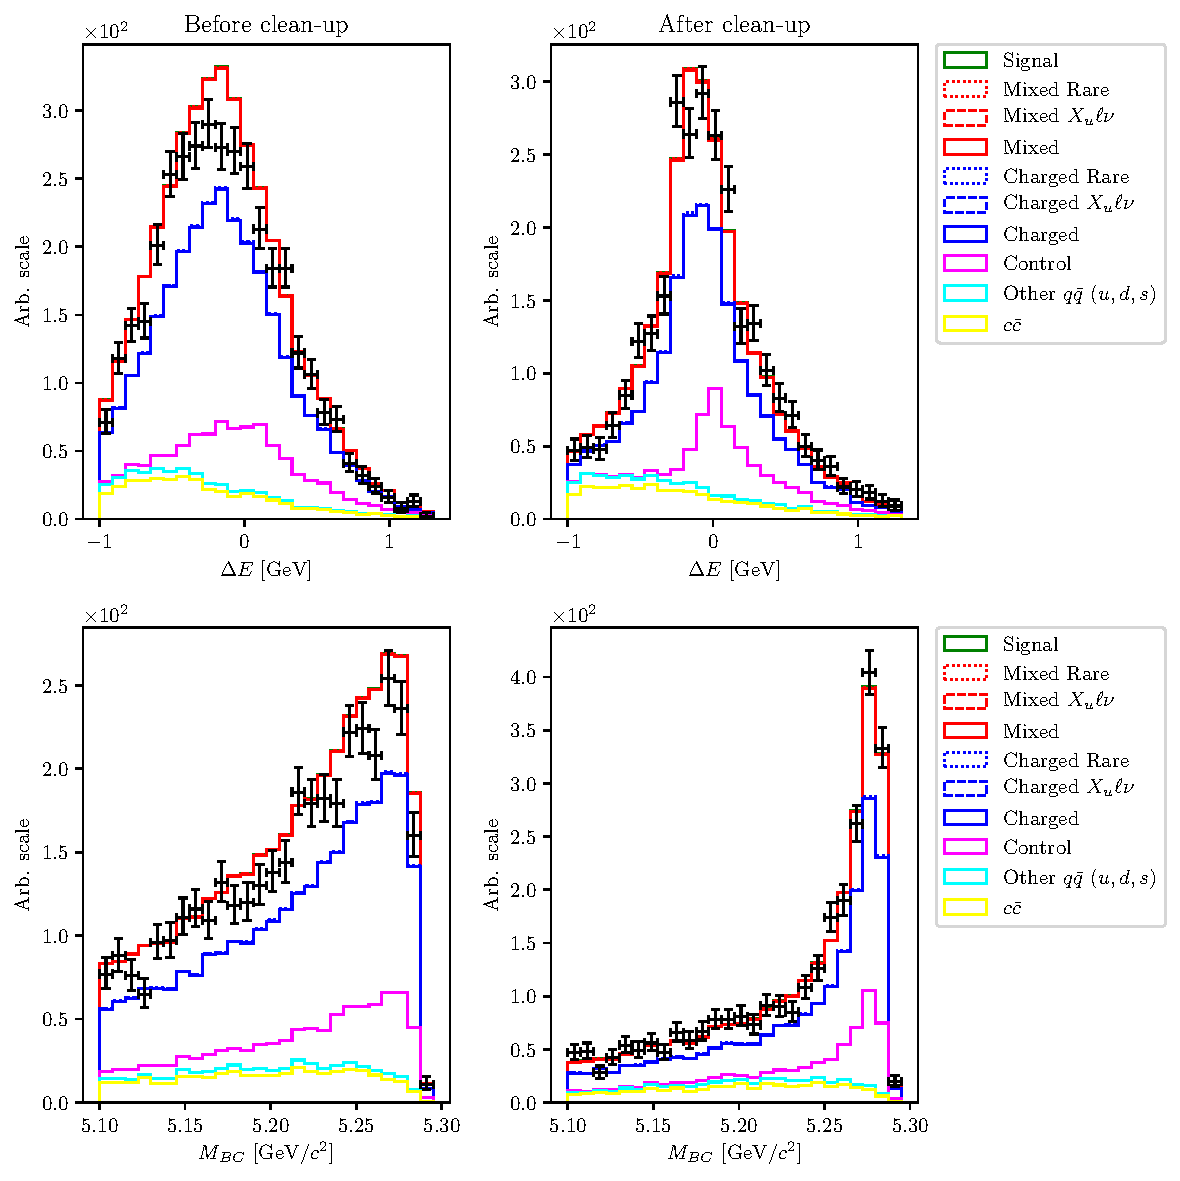
\includegraphics[width=\textwidth]{fig/roe_val}
	\column{0.4\textwidth}
	\begin{block}{}
	\begin{itemize}
		\item We validate the ROE clean-up procedure on the \textcolor{magenta}{control mode}
		\item ROE clean-up performs well on MC as well as on Daa
		\item The clean-up procedure does not introduce differences between MC and Data
	\end{itemize}
	\end{block}
\end{columns}


\end{frame}



%----------------------------------------------------------------------------------------

\begin{frame}[t]{Analysis VII -- Background Suppression}
\vspace{-3mm}
\small 

In order to further suppress various sources of background, we use \textit{machine learning algorithms}:\\
\vspace{1mm}
These algorithms take multiple properties of candidates as input and produce an output variable, similar to a signal probability\\
\vspace{1mm}
Boosted Decision Trees (BDT) algorithms are commonly used in the field

\only<1>{
\begin{block}{Continuum Suppression}
	\begin{itemize}
		\item Events of the form $e^+e^- \to q \bar q,$ where $q \in [u, d, s, c]$
		\item Energy and momentum distribution of such events differ from $e^+e^- \to B \bar B$ events
	\end{itemize}
\end{block}

\begin{block}{$B \bar B$ Suppression}
	\begin{itemize}
		\item Deeper look into the properties of the signal decay enable separation of signal from other $e^+e^- \to B \bar B$ events
	\end{itemize}
\end{block}
}

\only<2>{
\vspace{-2mm}
\begin{center}
	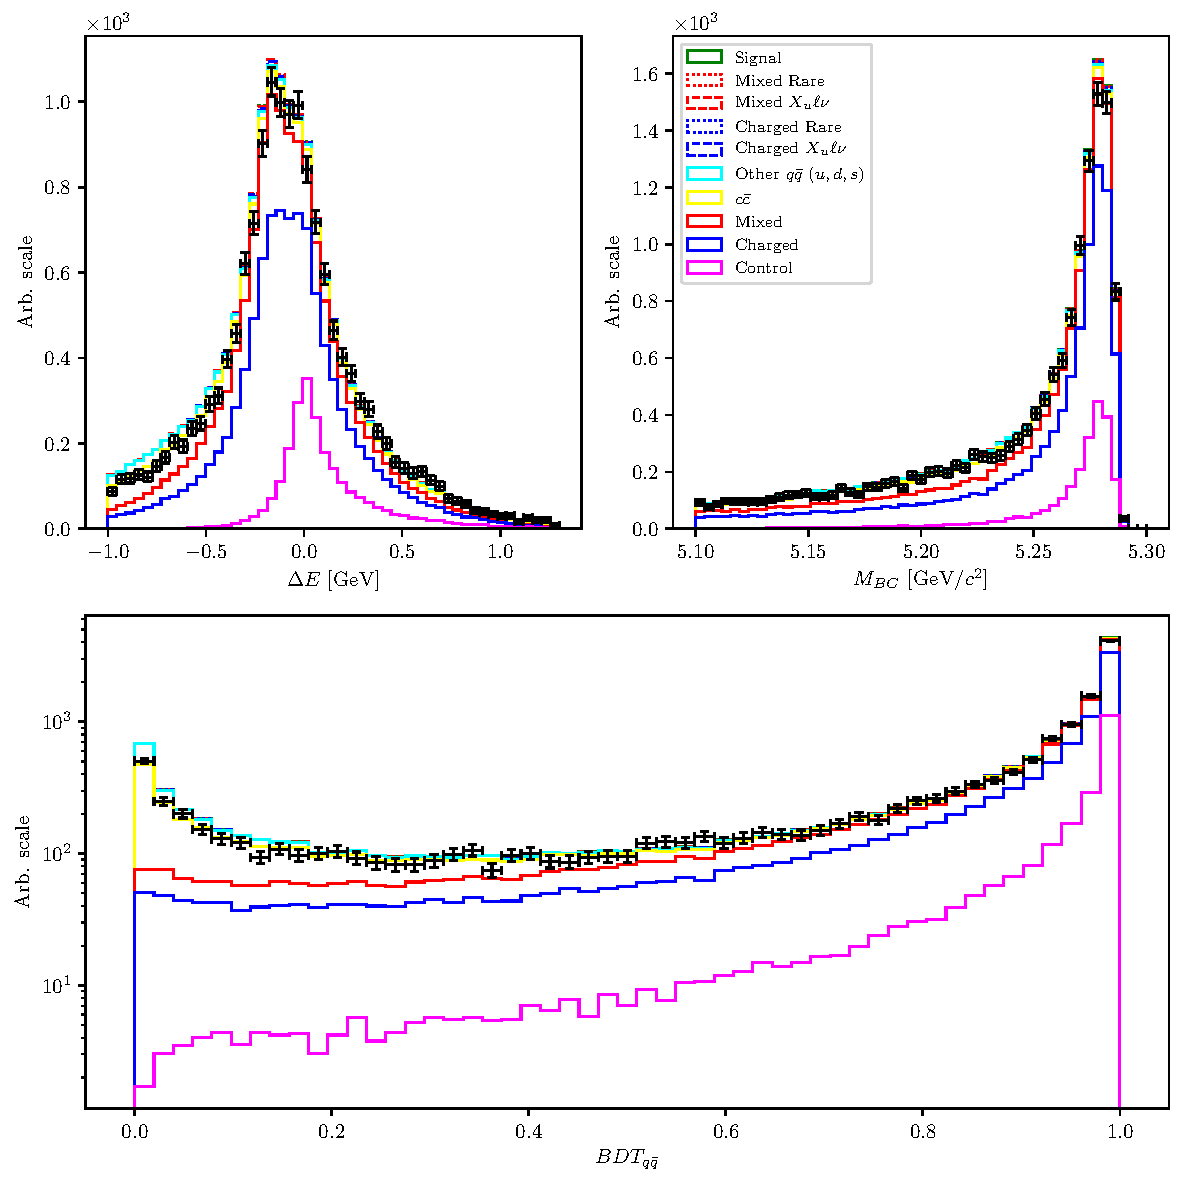
\includegraphics[width=0.8\textwidth, trim={0 0 0  8.5cm},clip]{fig/onres_control}
\end{center}
\vspace{-2mm}
Continuum (left) and $B \bar B$ (right) suppression BDT variable. Signal is more likely distributed on the right side of the variables.
}

\end{frame}

%----------------------------------------------------------------------------------------

\begin{frame}[t]{Analysis VIII -- Final Selection}
\vspace{-3mm}
\small

Sample composition after background suppression:
$$N_{\mathrm{sig}} = 264,\quad \frac{N_{\mathrm{sig}}}{N_{\mathrm{bkg}}} = 1.33\E{-2}$$

\begin{center}
	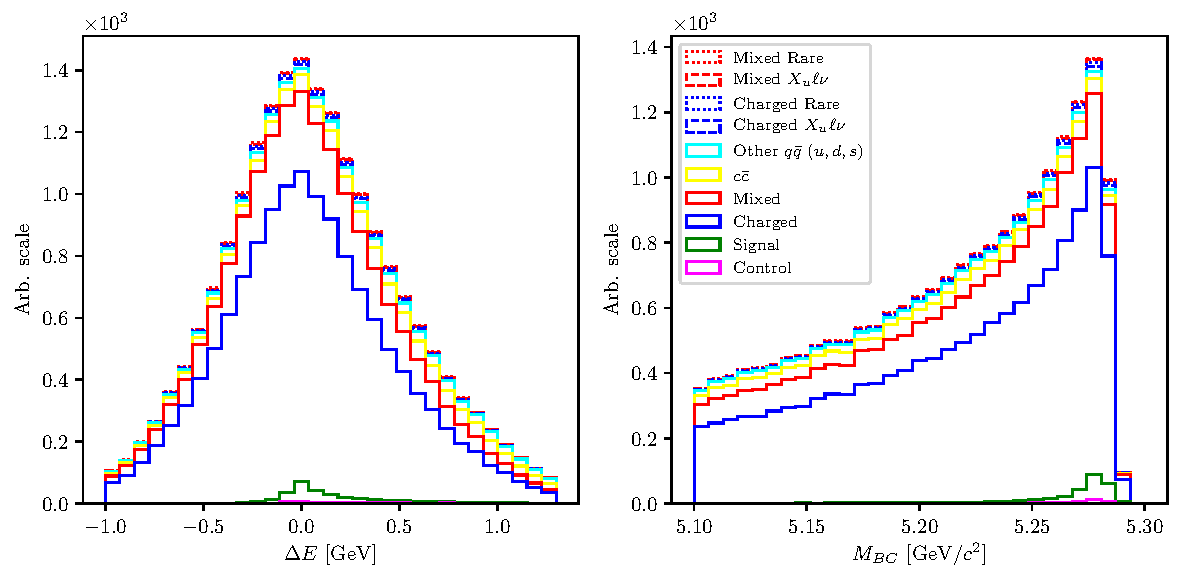
\includegraphics[width=\textwidth]{fig/opt_uBB_si}
\end{center}



\end{frame}




%----------------------------------------------------------------------------------------
\section{Parameter Extraction} 
%----------------------------------------------------------------------------------------

\begin{frame}[t]{Overview}
\only<1>{\tocforsect{5}{sectionstyle=shaded,subsectionstyle=shaded}}
\end{frame}


%----------------------------------------------------------------------------------------

\begin{frame}[t]{Parameter Extraction I -- Fit Method}
\vspace{-5mm}
\small

\begin{block}{}
	\begin{itemize}
		\item Define "templates" which describe distribution shapes (signal, background, $\dots$)
		\item For each histogram bin define Poisson probability for it's content w.r.t. the measurement
		\item Obtain the combination of template yields which maximise the probability
	\end{itemize}
\end{block}

\begin{columns}
	\column{0.4\textwidth}
	Templates in the signal fit:
	\begin{itemize}
		\item signal
		\item continuum
		\item well-defined sources $\to$\\of background
		\item other $B \bar B$ background
	\end{itemize}
	\column{0.6\textwidth}
	\begin{itemize}
		\tiny
		\item control decay,
		\item $B \to \bar{D} {}^* \ell^+ \nu,~D^0 \to K^-K^+$,
		\item $B \to \bar{D} {}^{(*)} \ell^+ \nu,~D^0 \to K^-\pi^+$,
		\item $B \to \bar{D} {}^{(*)} \ell^+ \nu,~D^0 \to K^-K^+\pi^0,~K^-\pi^+\pi^0$,
		\item $B \to \bar{D} {}^{(*)} \ell^+ \nu,~D^0 \to K^-\ell^+\nu$,
		\item $B^0 \to D^{(*)-} \ell^+ \nu,~D^+ \to K^-K^+\pi^+,~K^-\pi^+\pi^+$,
		\item other $B \to \bar D {}^{(*)} \ell^+ \nu$ decays,
	\end{itemize}
\end{columns}

\vspace{2mm}
{\color{red}Yields of all templates are floated, except in the well-defined cases, where yields are constrained by world measurements.}

\end{frame}


%----------------------------------------------------------------------------------------

\begin{frame}[t]{Parameter Extraction II -- Control Fit Results}
\vspace{-3mm}
\small

Results of the control decay fit to DATA

\begin{columns}
	\column{0.6\textwidth}
	\vspace{-2mm}
	\begin{center}
		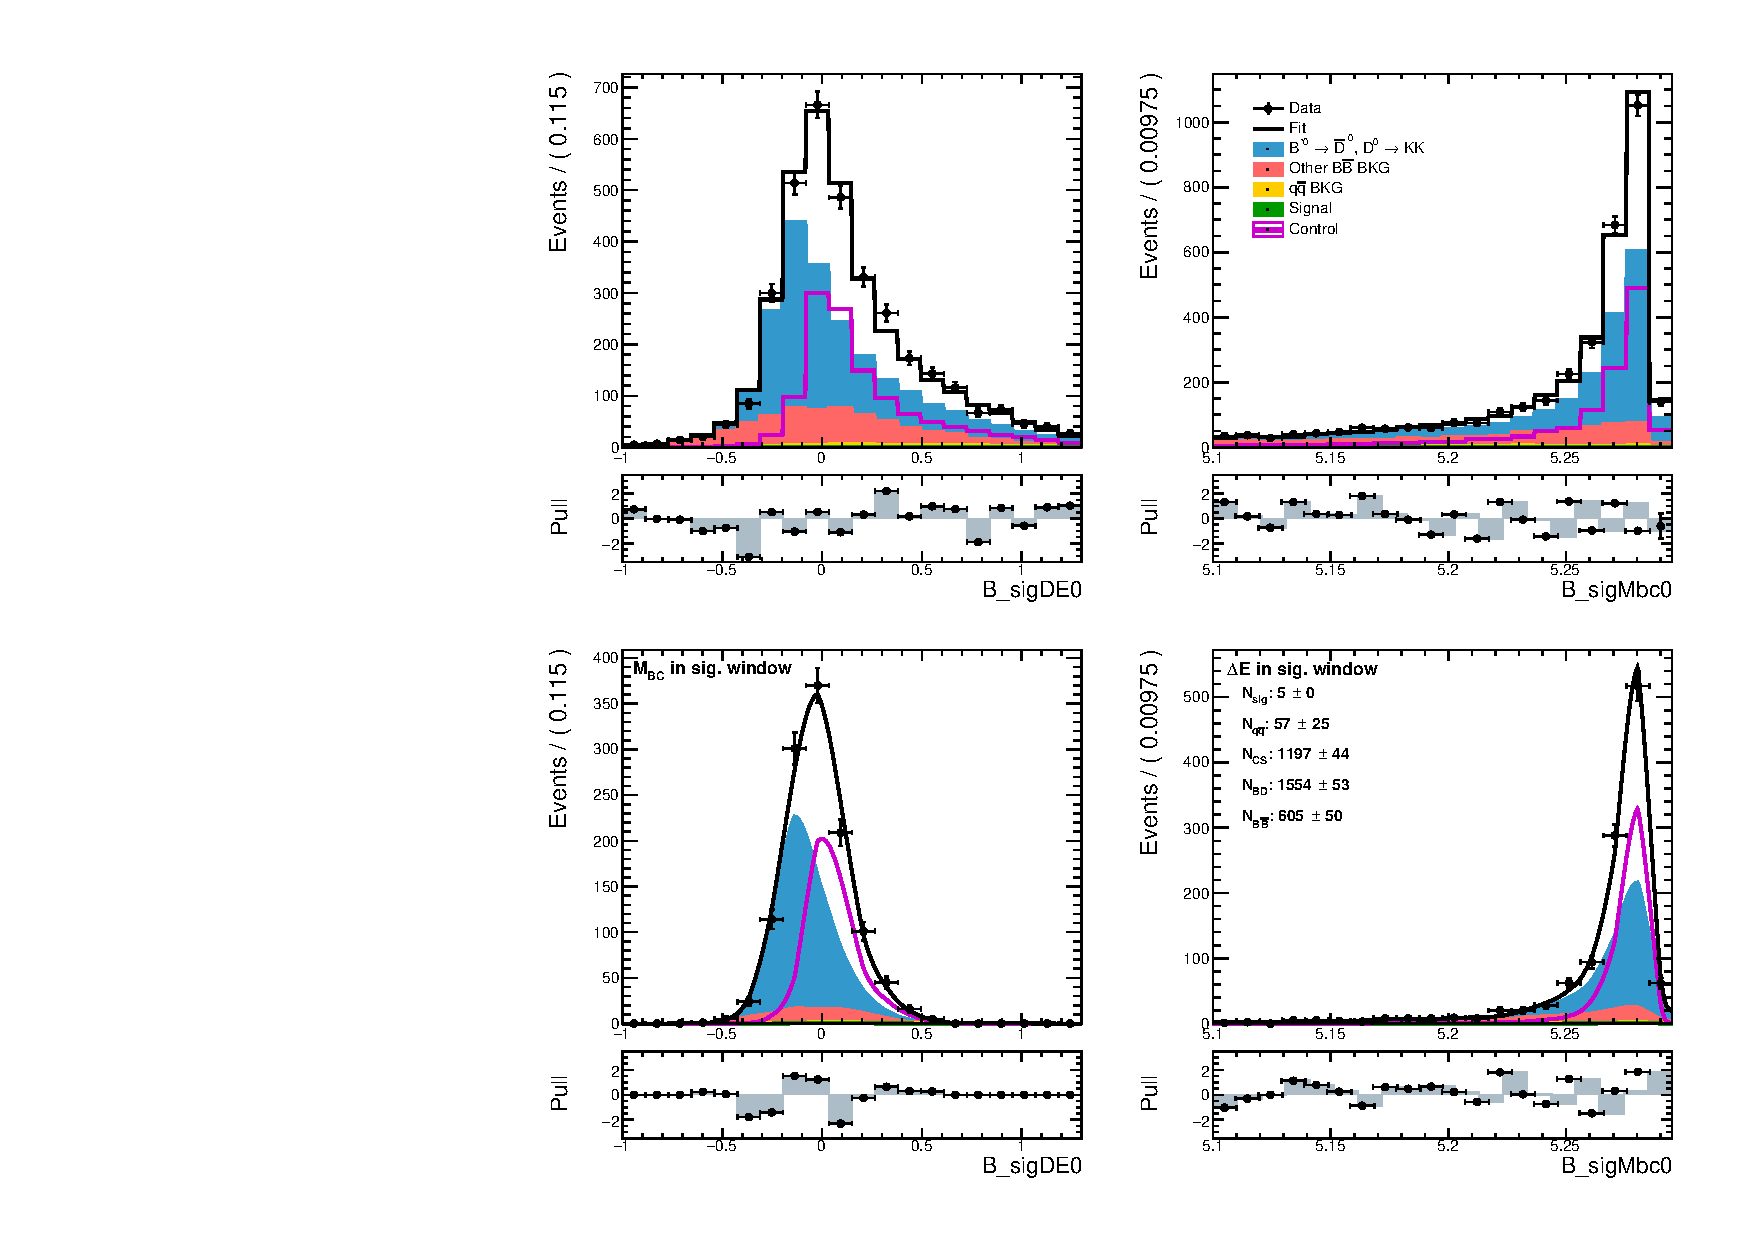
\includegraphics[width=\textwidth]{fig/cs_fit_data}
	\end{center}
	
	\column{0.4\textwidth}
	\begin{block}{}
		\begin{itemize}
			\item Plot: White part represented by the \textcolor{magenta}{control decay}, which is drawn separately
			\item \textcolor{blue}{Blue contribution} mostly from $B \to D^* \ell \nu$, shift in $\Delta E$ due to a missing particle ($\pi^\pm$)
			\item Templates are appropriately summed to best fit the measurement
			\item The fit behaves well, no strange artefacts in pulls 
		\end{itemize}
	{\tiny pulls $\propto$ differences between the function and the points}
	\end{block}
\end{columns}


\end{frame}

%----------------------------------------------------------------------------------------

\begin{frame}[t]{Parameter Extraction II -- Control Fit Results}
\vspace{-3mm}
\small

Control decay branching ratio measurement
\vspace{-2mm}
\begin{center}
	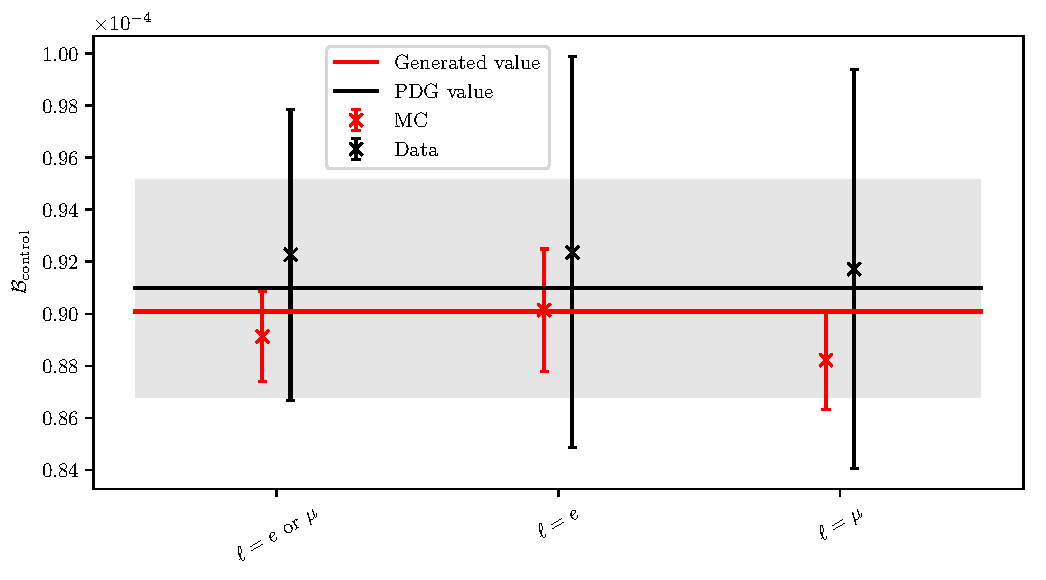
\includegraphics[width=0.9\textwidth]{fig/br_plot}
\end{center}
\vspace{-2mm}
\textcolor{turtlegreen}{The simulated and measured values of the control decay branching ratio seems to agree well with the generated value and the world average from PDG (\url{http://pdglive.lbl.gov}).}

\end{frame}

%----------------------------------------------------------------------------------------

\begin{frame}[t]{Parameter Extraction III -- Signal Fit Results}
\vspace{-3mm}
\small

Results of the signal decay fit to DATA
\begin{columns}
	\column{0.6\textwidth}
	\vspace{-2mm}
	\begin{center}
		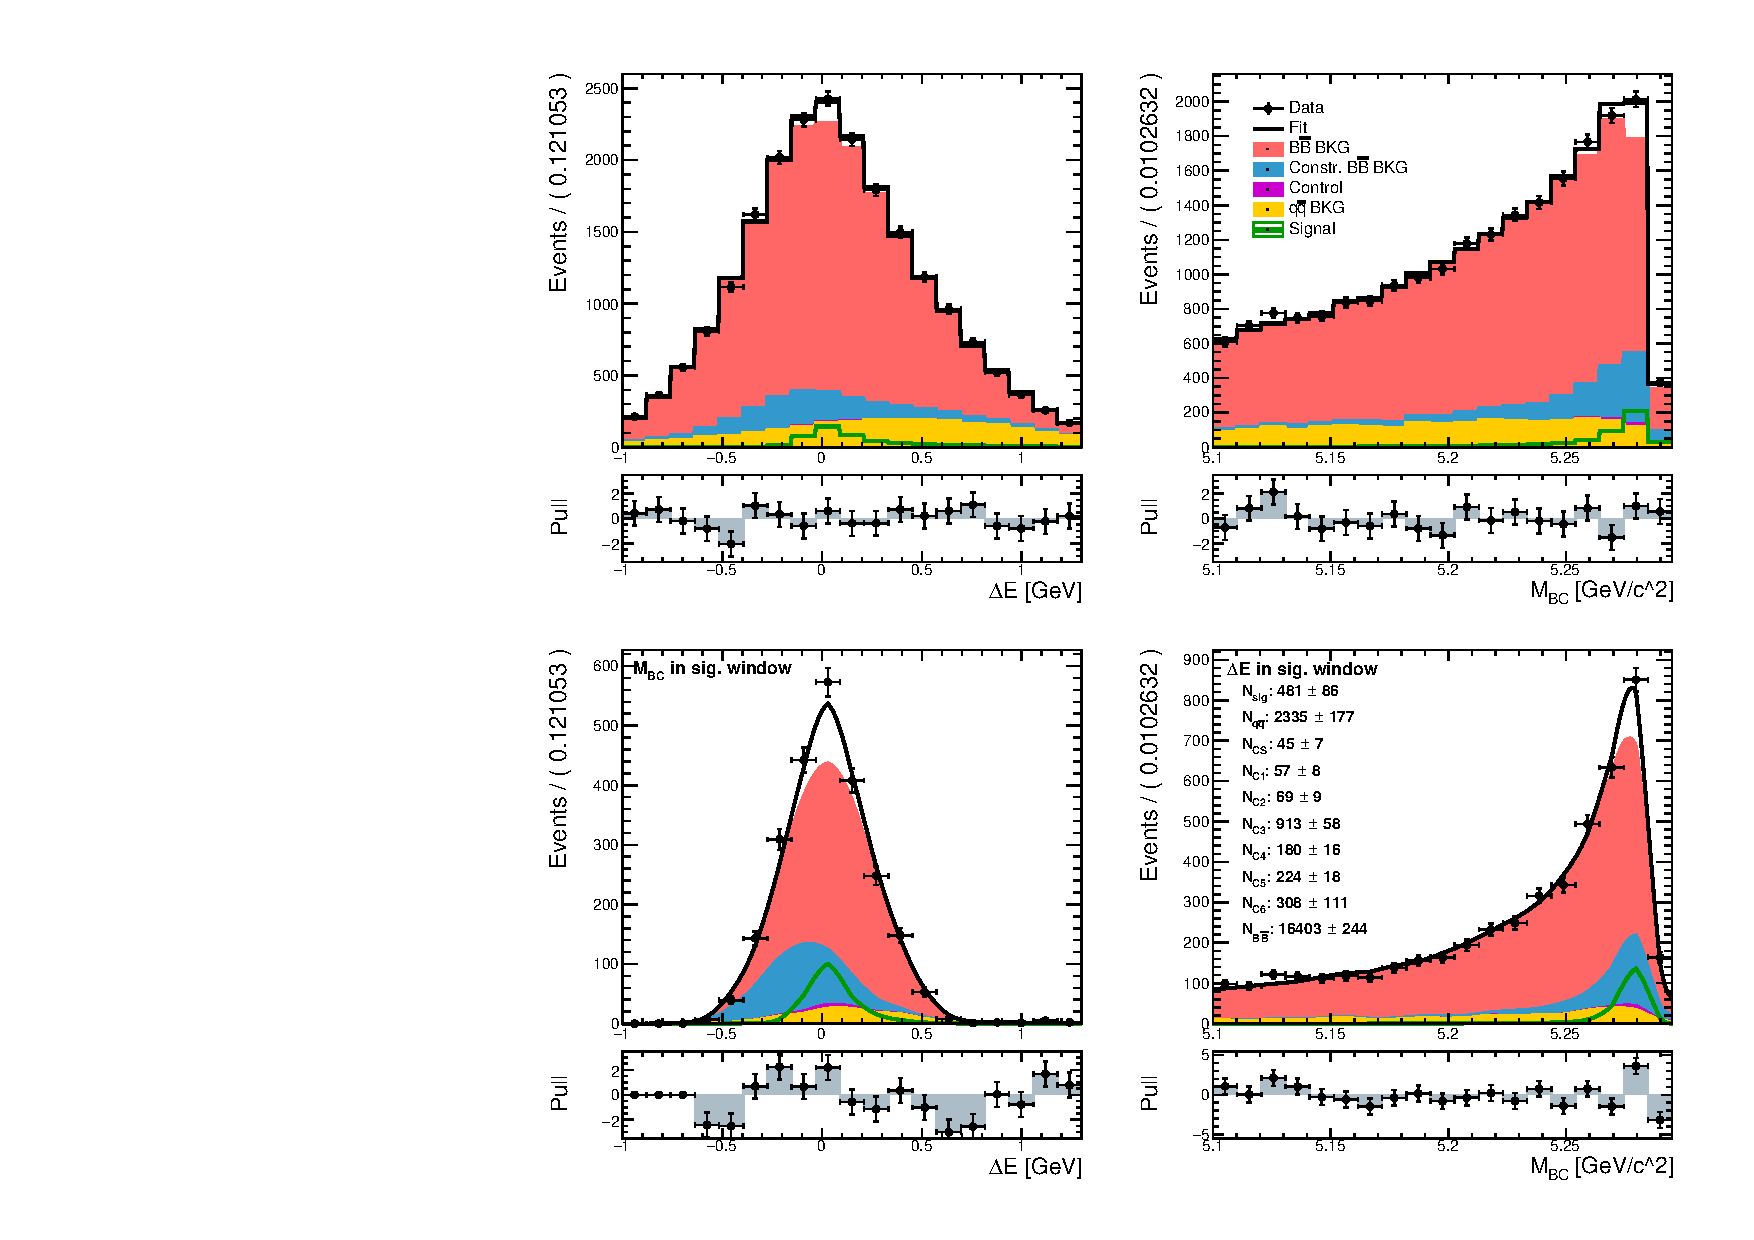
\includegraphics[width=\textwidth]{fig/sig_fit_data}
	\end{center}
	
	\column{0.4\textwidth}
		\vspace{-7mm}
		\begin{block}{}
		White part represented by the \textcolor{green}{signal decay}, which is drawn separately
	\end{block}
\vspace{-4mm}
	\begin{table}[H]
		\centering
		\begin{tabular}{l|l}
			Category & Fit Yield \\
			\toprule
			Signal & $491 \pm 86$ \\
			$q \bar q$ bkg & $ 2385 \pm 181 $ \\
			$C_0$ & $ 45 \pm 7 $ \\
			$C_1$ & $ 57 \pm 8 $\\
			$C_2$ & $ 69 \pm 9 $ \\
			$C_3$ & $ 907 \pm 57 $ \\
			$C_4$ & $ 178 \pm 16 $ \\
			$C_5$ & $ 224 \pm 18 $ \\
			$C_6$ & $ 322 \pm 108 $ \\
			Other $B \bar B$ bkg & $ 16382 \pm 247 $ \\
			\bottomrule
		\end{tabular}
	\end{table}
\end{columns}


\end{frame}

%----------------------------------------------------------------------------------------

\begin{frame}[t]{Parameter Extraction III -- Signal Fit Results}
\vspace{-3mm}
\small

Signal fit to measured data and 10 equal samples of simulated data (streams)
\vspace{-2mm}
\begin{center}
	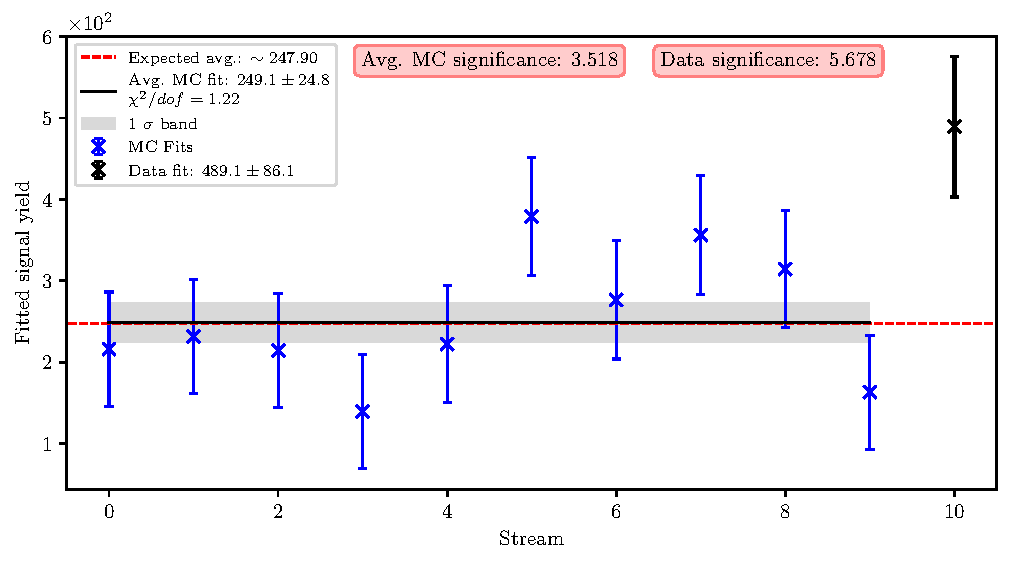
\includegraphics[width=\textwidth]{fig/sig_global}
\end{center}

\textcolor{turtlegreen}{Much more signal in measured data than expected from simulation!}	

\end{frame}

%----------------------------------------------------------------------------------------

\begin{frame}[t]{Parameter Extraction IV -- Signal Distributions}
\vspace{-3mm}
\small

\begin{columns}
	\column{0.56\textwidth}
	\begin{center}
		\begin{tikzpicture}
		\node at (0,0) {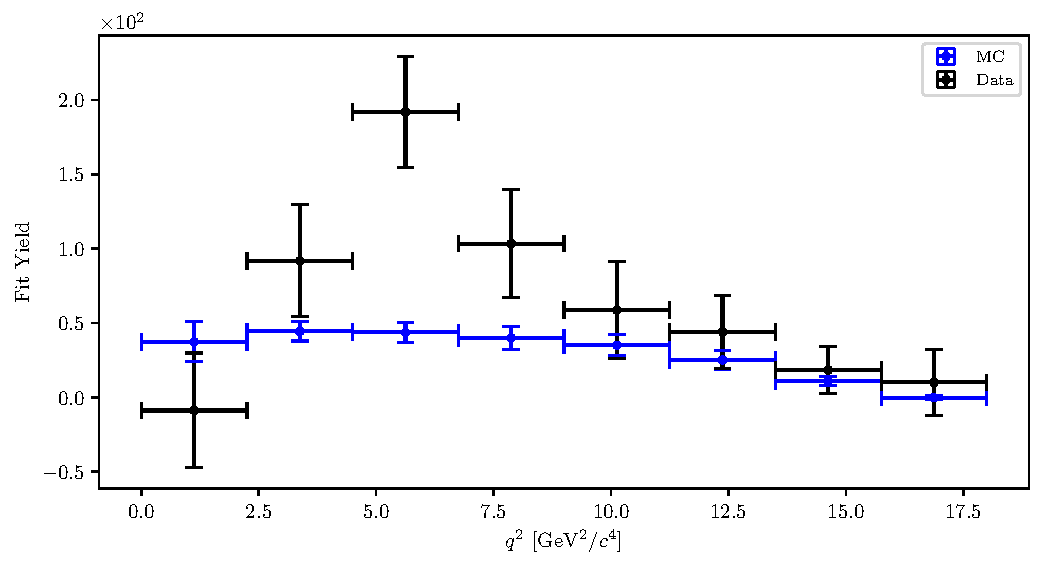
\includegraphics[width=0.9\textwidth]{fig/sig_q2_all}};
		\node at (0,3.5){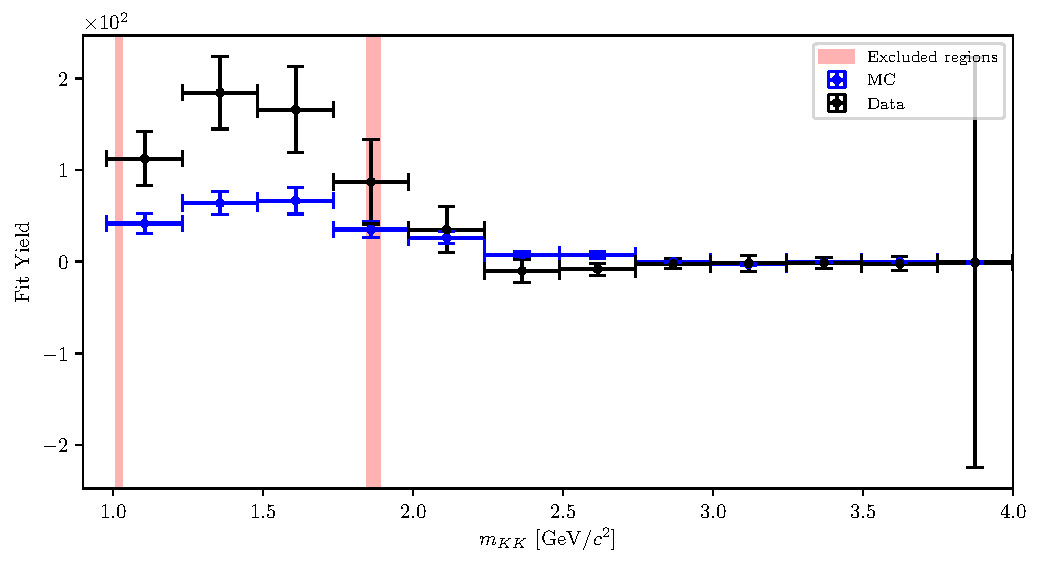
\includegraphics[width=0.9\textwidth]{fig/sig_mKK_all}};
		
		\node at (1.5,3.8) {
			\begin{tabular}{l}
			DATA\\
			\textcolor{blue}{MC}\\
			\end{tabular}
		};
		
		
		\draw[thick, ->] (0.9,4.05) to [out=180,in=0] (-1.2,4.5);
		\draw[blue, thick, ->] (0.9,3.65) to [out=180,in=60] (-1.6,3.4);
		%\draw[thick, ->] (0.3,-3.4) to [out=180,in=270] (-3.8,0);
		%
		%\draw[thick, turtlegreen, ->] (4,3) to [out=-90,in=0] (2.2,1);
		%\draw[thick, turtlegreen, ->] (2.6,3.7) to [out=180,in=0] (0.2,3);
		
		
		\end{tikzpicture}
	\end{center}
	\column{0.4\textwidth}
	\begin{block}{}
		\begin{itemize}
			\item Invariant mass of two kaons
			\item Distributions are similar
			\item Signal much more abundant in DATA
		\end{itemize}
	\end{block}
\begin{block}{}
	\begin{itemize}
		\item $\mathrm{q}$ is the 4-momentum transferred to the lepton pair
		\item Distributions are quite different
		\item Signal much more abundant in DATA
	\end{itemize}
\end{block}
\end{columns}

Such measurements help improve future models and minimize difference between data and simulations. 



\end{frame}

%----------------------------------------------------------------------------------------
\section{Systematic Uncertainties} 
%----------------------------------------------------------------------------------------

\begin{frame}[t]{Overview}
\only<1>{\tocforsect{6}{sectionstyle=shaded,subsectionstyle=shaded}}
\end{frame}

%----------------------------------------------------------------------------------------

\begin{frame}[t]{Systematic Uncertainties I -- Model Dependency}

\vspace{-3mm}
\small

\begin{itemize}
	\item Largest source of uncertainty in this analysis
	\item \texttt{ISGW2} model for signal decay is not the most reliable, try to not depend on it
	\item Three additional signal models are used to estimate dependency, used as substitute templates
	\item Different models have different signal efficiencies
\end{itemize}
\vspace{-2mm}

	\begin{center}
		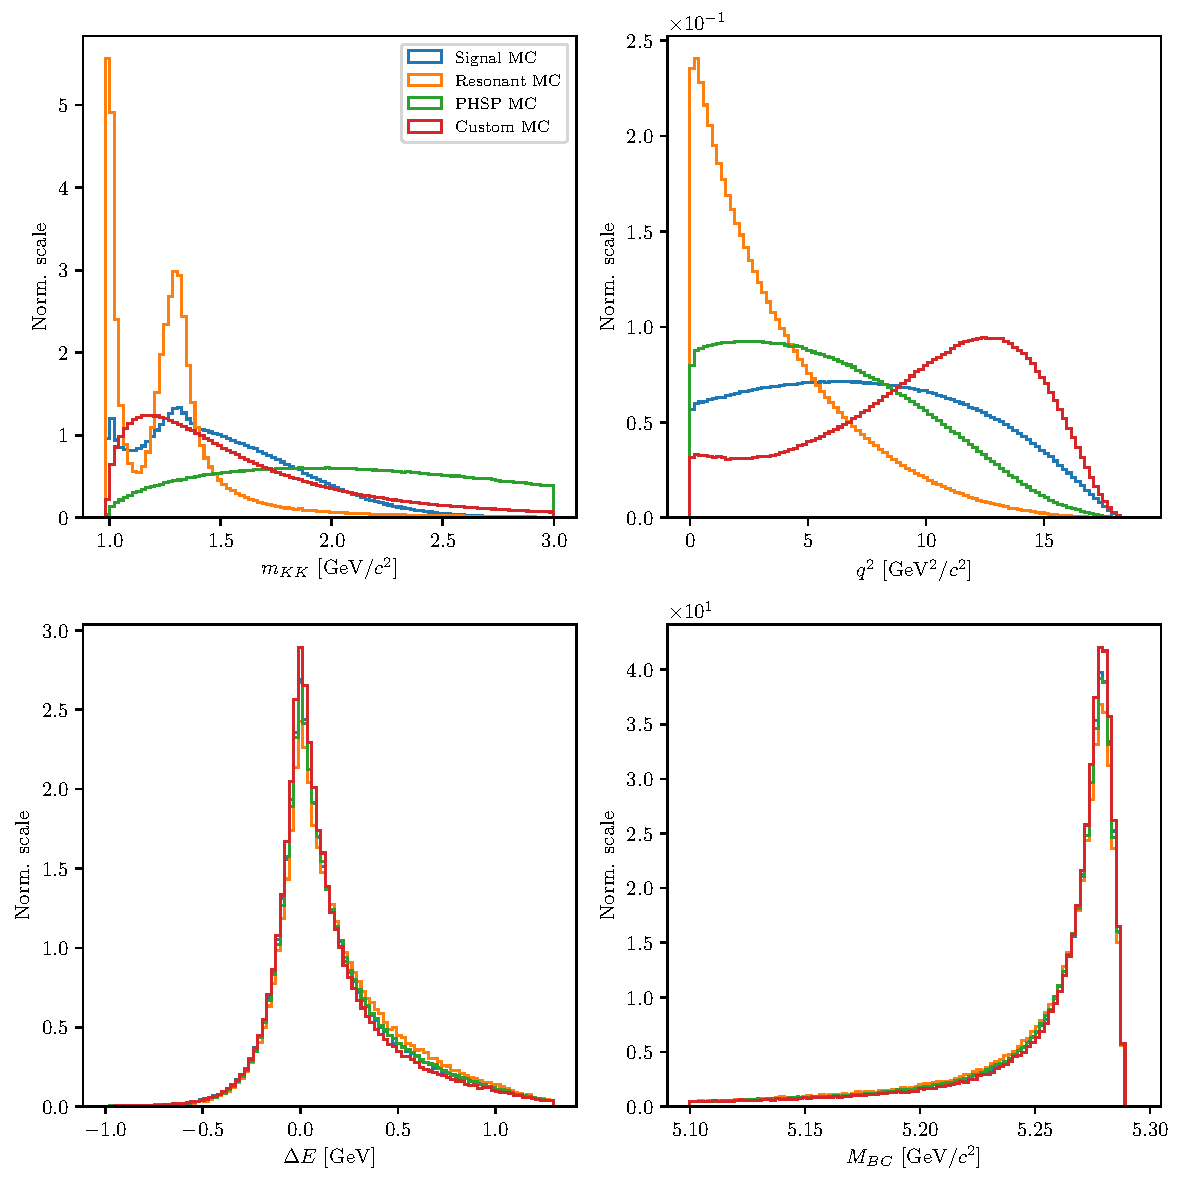
\includegraphics[width=0.8\textwidth, trim={0 10cm 0 0},clip]{fig/model_cases}
	\end{center}	


\end{frame}

%----------------------------------------------------------------------------------------

\begin{frame}[t]{Systematic Uncertainties I -- Model Dependency}

\vspace{-3mm}
\small

\begin{center}
	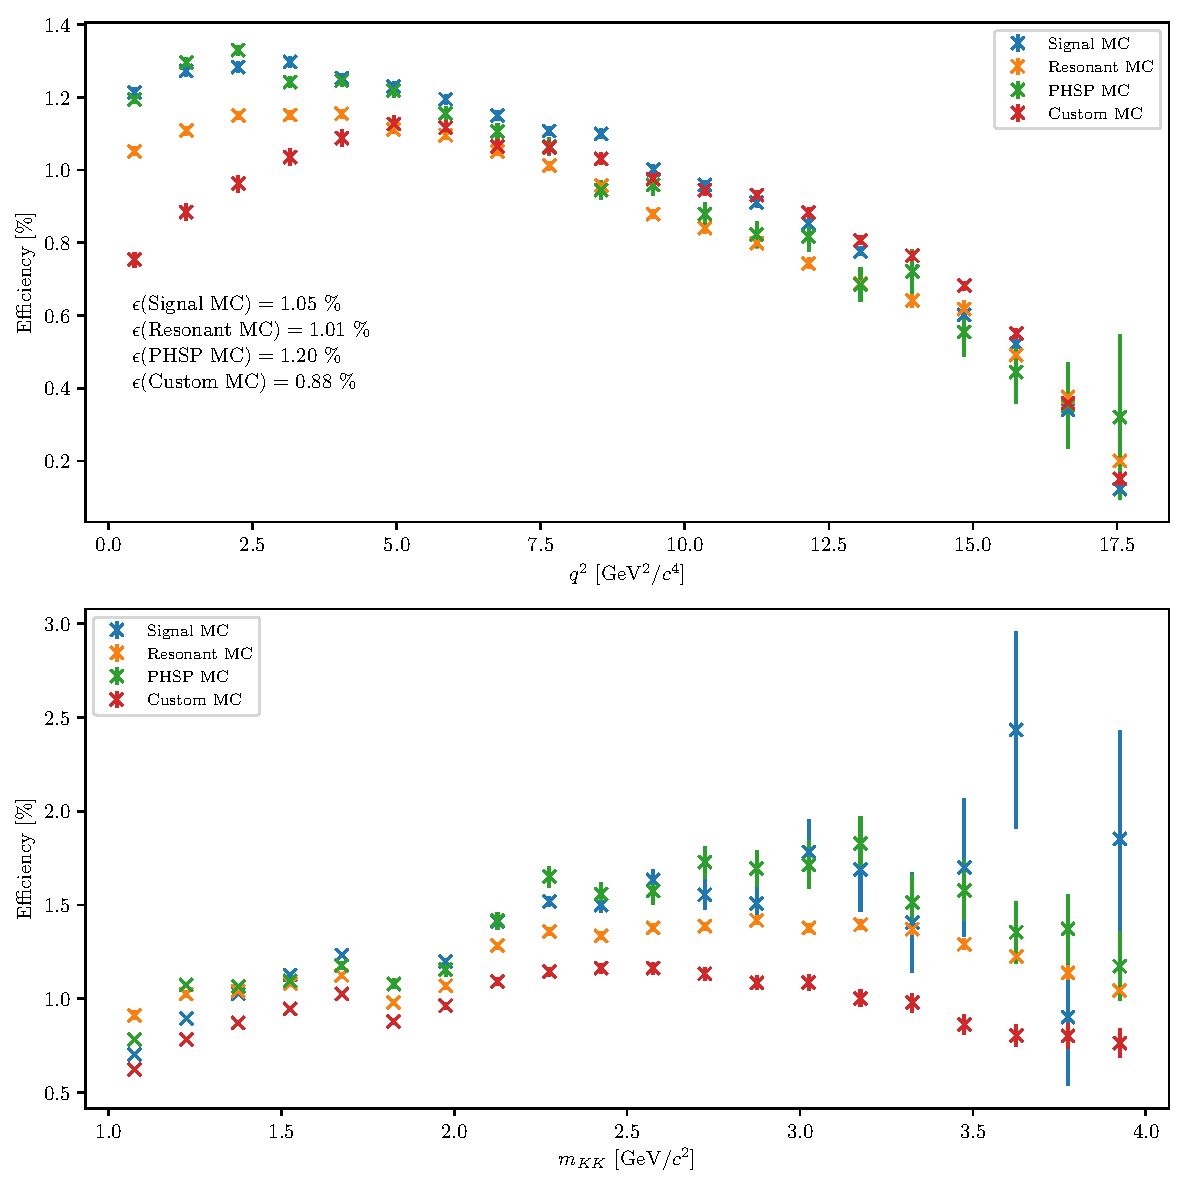
\includegraphics[width=0.65\textwidth]{fig/efficiencies}
\end{center}	


\end{frame}

%----------------------------------------------------------------------------------------

\begin{frame}[t]{Systematic Uncertainties II -- All Sources}

\vspace{5mm}

\begin{table}[H]
	\centering
	\begin{tabular}{l|c|c}
		Source & Absolute ($\sigma$) & Relative ($\delta)~[\%]$ \\
		\toprule
		PID & $10$ & $2.0$ \\
		Fit Bias & $ {}^{+7}_{-10}$ & ${}^{+1.5}_{-2.0}$ \\
		Gaussian Constraints & $26$ & $5.4$ \\
		Template Smearing & ${}^{+41}_{-33}$ & ${}^{+8.3}_{-6.7}$ \\
		Template Offset & ${}^{+41}_{-31}$ & ${}^{+8.4}_{-6.3}$ \\
		Finite MC Effects & $26$ & $5.3$ \\
		MVA Selection & $5$ & $1.0$\\
		Model Shape & ${}^{+45}_{-39}$ & ${}^{+9.3}_{-8.0}$ \\
		Model Efficiency & ${}^{+70}_{-79}$ & ${}^{+14.3}_{-16.2}$ \\
		\midrule
		Total & ${} ^{+109}_{-107}$ & ${}^{+22.2}_{-21.9}$ \\
		\bottomrule
	\end{tabular}
\end{table}


\end{frame}

%----------------------------------------------------------------------------------------

%----------------------------------------------------------------------------------------
\section{Results} 
%----------------------------------------------------------------------------------------

\begin{frame}[t]{Overview}
\only<1>{\tocforsect{7}{sectionstyle=shaded,subsectionstyle=shaded}}
\end{frame}

%----------------------------------------------------------------------------------------

\begin{frame}[t]{Results I -- Branching Ratio of Signal Decay}

Calculated branching ratio from simulated data is:
$$
\mathcal{B}^{\mathrm{MC}}(B^+ \to K^+ K^- \ell^+ \nu) = (1.55 \pm 0.15)\E{-5},
$$


And on data, after taking all uncertainties into account:
$$
\mathcal{B}(B^+ \to K^+ K^- \ell^+ \nu) = (3.04 \pm 0.51 \pm {}^{+0.67}_{-0.66})\E{-5},
$$
where the first and the last error are statistical and systematic, respectively.\\

\vspace{1cm}
\textcolor{turtlegreen}{Almost a factor of 2 difference!}

\end{frame}

%----------------------------------------------------------------------------------------

\begin{frame}[t]{Results II -- Signal Significance}
\vspace{-3mm}
\small

\begin{itemize}
	\item Profile likelihood gives the value of likelihood at different expected yields of signal, used for significance estimation
	\item Statistical significance corresponds to $6.3\sigma$
	\item Systematic uncertainties are incorporated via a convolution
	\item Overall signal significance $4.6\sigma~\to$ evidence!
\end{itemize}

\vspace{-2mm}

\begin{center}
	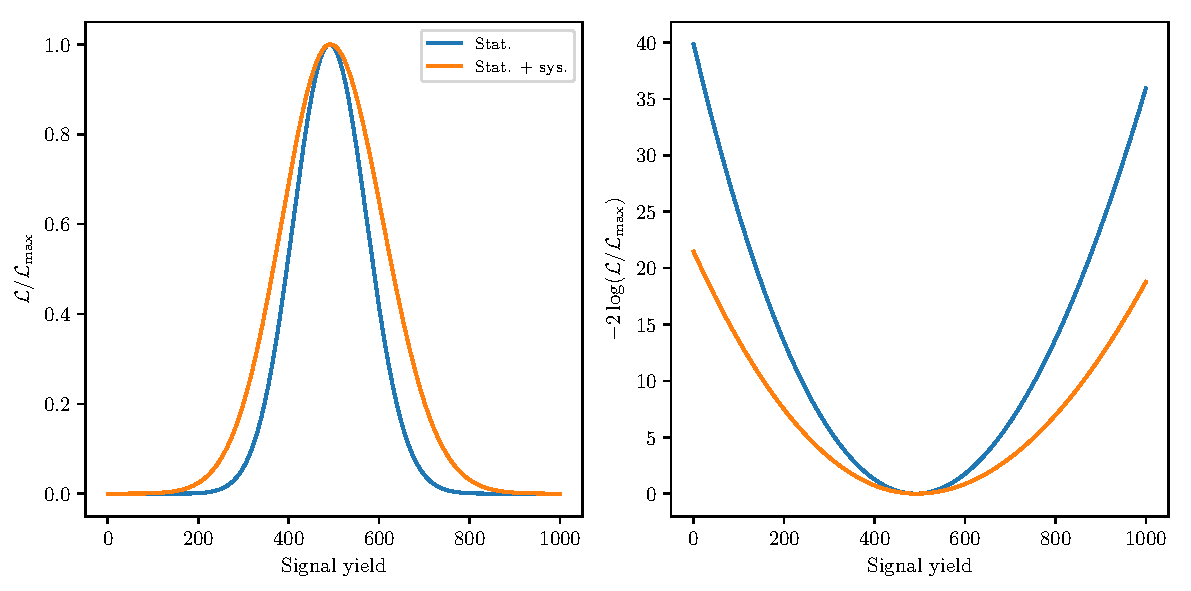
\includegraphics[width=0.9\textwidth]{fig/significance}
\end{center}

\end{frame}


%----------------------------------------------------------------------------------------

\begin{frame}[t]{Summary}
\begin{block}{}
\begin{itemize}
	\item Improvement in the untagged method with the ROE clean-up
	\item Demonstration of the aid of machine learning algorithms in such analyses
	\item Evidence for the previously unstudied decay mode $B^+ \to K^+ K^- \ell^+ \nu_\ell$ (and c.c.), with additional insight into signal distributions
	\item Current studies underestimate the amount of charmless semileptonic $B$ meson decays with kaons in the final state. Future analyses can take such decay modes into account and produce more quantitative results.
\end{itemize}
\end{block}
\end{frame}

%----------------------------------------------------------------------------------------

\begin{frame}[t]
\begin{center}
	{\Huge Thank you!}
	\vspace{2mm}	
	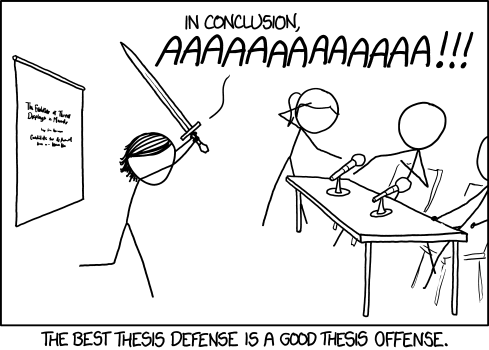
\includegraphics[width=0.8\textwidth]{fig/thesis_defense}
\end{center}
	\vspace{-2mm}	
\url{https://xkcd.com/1403/}
\end{frame}


%----------------------------------------------------------------------------------------

\appendix
\backupbegin

\begin{frame}[t]
\vspace{0.4\textheight}
\begin{center}
	{\Huge BACKUP}
\end{center}
\end{frame}

%----------------------------------------------------------------------------------------


\begin{frame}[t]{Backup -- Selection Criteria}

\vspace{-3mm}
\small

Selection:
\begin{itemize}
	\item FSP particles:
	\begin{itemize}
		\item electrons: $\vert d_0 \vert < 0.1\e{cm},\,\vert z_0 \vert < 1.5\e{cm},\,p>0.6\e{GeV}/c,\,p_{CMS}\in[0.4,\,2.6]\e{GeV}/c,\,eID>0.9,$
		\item muons: $\vert d_0 \vert < 0.1\e{cm},\,\vert z_0 \vert < 1.5\e{cm},\,p_{CMS}\in[0.6,\,2.6]\e{GeV}/c,\,\mu ID>0.97,$
		\item kaons: $\vert d_0 \vert < 0.15\e{cm},\,\vert z_0 \vert < 1.5\e{cm},\,p_{CMS} < 2.5\e{GeV}/c,\,K/\pi~ID>0.6,\,K/p~ID>0.1,$
	\end{itemize}
	\item $B$ meson candidates:
	\begin{itemize}
		\item standard selection: $P(\chi^2,\,DOF) > 6\E{-3},\,\vert \cos \theta_{BY} \vert < 1.05,\,\vert m_{miss}^2\vert<0.975\e{GeV}/c^2,$
		\item fit region selection: $\Delta E \in [-1.0,1.3]\e{GeV},\,M_{BC} \in [5.1,5.295]\e{GeV}/c^2,$
		\item signal region selection: $\vert \Delta E \vert < 0.126\e{GeV},\,M_{BC} > 5.271\e{GeV}/c^2,$
		\item charge categorization: $q_{B^\pm}q_{B^\mp} = -1.$
	\end{itemize}
\end{itemize}


\end{frame}

%----------------------------------------------------------------------------------------
\begin{frame}[t]{Backup -- Generated $m_{KK}$ Distribution}
\vspace{-3mm}
\small

\begin{figure}[H]
	\centering
	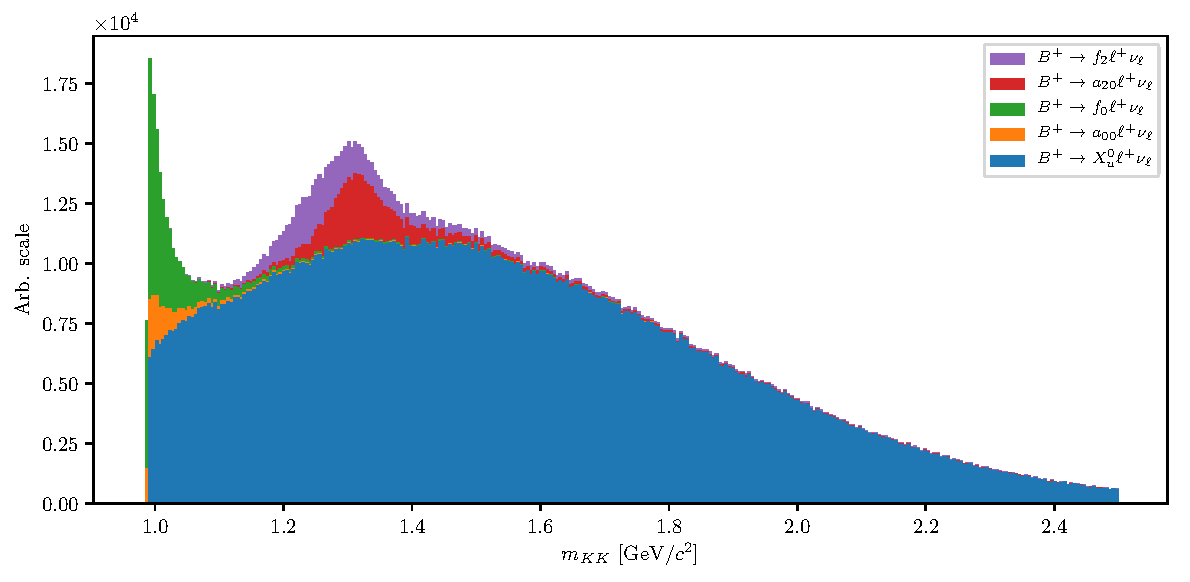
\includegraphics[width=\linewidth]{fig/KKlnu_src}
	\caption{Invariant mass of the $KK$ pair from various contributions of the MC generator. The light unflavored states have small contributions with resonant structure, while $KK$ pairs from the $X_u^0$ state are more abundant and follow a wider and smoother distribution.}
\end{figure}

\end{frame}

%----------------------------------------------------------------------------------------
\begin{frame}[t]{Backup -- Other $KK$ decays}
\vspace{-3mm}
\small
\begin{table}[H]
	\centering
	\begin{tabular}{l|c||l|c}
		Channel & Ratio $[\%]$ & Channel & Ratio $[\%]$ \\
		\toprule 
		$K^+ K^-$ & 28.14 & $K^+ K^- \rho^0$ & 1.93 \\
		$K^+ K^- \pi^0$ & 8.94 & $K^+ \bar{K}{}^0 \rho^-$ & 1.84 \\
		$K^+ \bar{K}{}^0 \pi^-$ & 8.71 & $K^0 K^- \rho^+$ & 1.83 \\
		$K^0 K^- \pi^+$ & 8.70 & $K^0 \bar K {}^0 \rho^0$ & 0.00 \\
		$K^+ K^- \pi^+ \pi^-$ & 4.15 &  $K^+ K^- \pi^0 \pi^0$ & 0.86 \\
		$K^0 \bar K {}^0$ & 3.32  & $K^+ K^- \pi^+ \rho^-$ & 0.69 \\
		$K^0 \bar K {}^0 \pi^0$ & 3.26 & $K^+ K^- \rho^+ \pi^-$ & 0.68 \\
		\midrule
		$K \bar K$ pair with $\eta$ & 7.08  & & \\
		$K \bar K$ pair with $\omega$ & 5.33  & & \\
		Other & 14.53  & & \\
		\bottomrule 
	\end{tabular}
	\caption{Relative branching fractions of $B \to KKX\ell \nu$ decays by channel.}
\end{table}

\end{frame}

%----------------------------------------------------------------------------------------
\begin{frame}[t]{Backup -- B2BII Tracks}
\vspace{-3mm}
\small
\begin{figure}[H]
	\centering
	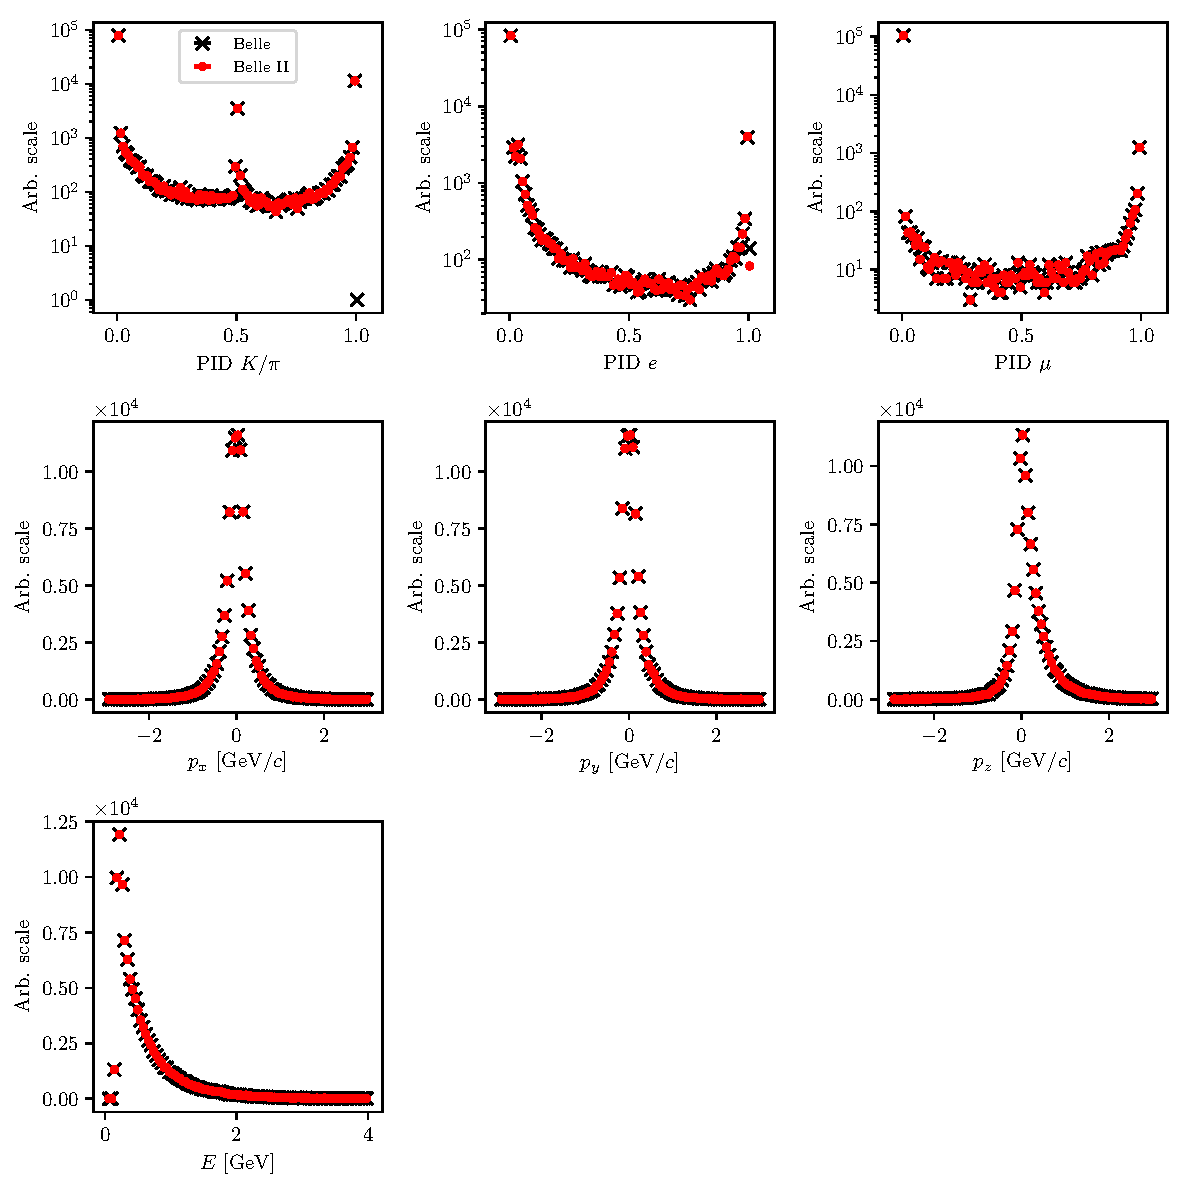
\includegraphics[width=0.5\linewidth]{fig/b2bii_tracks}
	\caption{Some of the more important physical properties of tracks for Belle and Belle II in the conversion process. The histograms seem to overlap and the conversion is assumed to be successful.}
	\label{fig:b2bii_tracks}
\end{figure}
\end{frame}

%----------------------------------------------------------------------------------------
\begin{frame}[t]{Backup -- B2BII Clusters}
\vspace{-3mm}
\small
\begin{figure}[H]
	\centering
	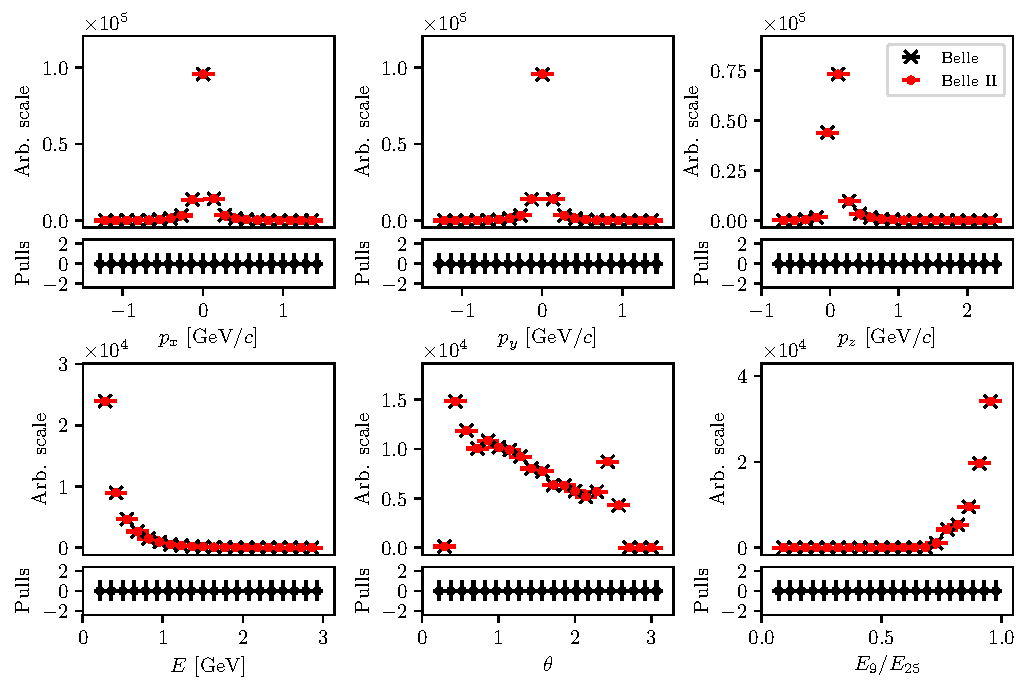
\includegraphics[width=\linewidth]{fig/b2bii_gammas}
	\caption{Some of the more important physical properties of photons for Belle and Belle II in the conversion process. The histograms seem to overlap and the conversion is assumed to be successful.}
	\label{fig:b2bii_gammas}
\end{figure}
\end{frame}

%----------------------------------------------------------------------------------------
\begin{frame}[t]{Backup -- $q^2$ Calculation}
\vspace{-3mm}
\small
\begin{figure}[H]
	\centering
	\includegraphics[width=0.8\linewidth]{fig/q2}
	\caption{Distributions of $q^2$ (left) and $q^2$ resolution (right) for various methods of $q^2$ calculation. The green distribution follows the procedure in \cite{VubCLEO}, the blue distribution takes into account the weighted average of the $B$ meson direction \cite{Ha:2010rf}, and the red and orange distributions are straight-forward calculations with available information in the reconstruction. The $q^2$ calculation in red assumes a resting $B$ meson in the CMS frame, and the calculation in orange uses the neutrino four-momentum summed up tracks and clusters in ROE.}
\end{figure}
\end{frame}

%----------------------------------------------------------------------------------------
\begin{frame}[t]{Backup -- Signal Window Definition}
\vspace{-3mm}
\small
\begin{figure}[H]
	\centering
	\includegraphics[width=\linewidth]{fig/sigWin}
	\caption{2D $FOM$ optimization of the signal region definition, where most of the perfectly reconstructed candidates are located.}
\end{figure}
\end{frame}

%----------------------------------------------------------------------------------------
\begin{frame}[t]{Backup -- ROE Clean-up Validation (Split)}
\vspace{-3mm}
\small
\begin{figure}[H]
	\centering
	\includegraphics[width=0.8\linewidth]{fig/roe_val_split}
	\caption{Distributions of $\Delta E$ (top) and $M_{BC}$ (bottom) split in bins of the charge product of the two $B$ mesons.}
\end{figure}
\end{frame}

%----------------------------------------------------------------------------------------
\begin{frame}[t]{Backup -- BDT for $B \bar B$ Suppression}
\vspace{-3mm}
\small
\begin{figure}[H]
	\centering
	\includegraphics[width=0.9\linewidth]{fig/bb_BDT}
	\caption{$B\bar B$ suppression classifier output for signal and various types of background for the standard $BDT$ classifier (left) and the $uBDT$ classifier (right). $B$ candidates from $B\bar B$ background events dominate the lower region, while signal and control candidates dominate in the upper region of the classifier output.}
\end{figure}
\end{frame}

%----------------------------------------------------------------------------------------
\begin{frame}[t]{Backup -- $B \bar B$ BKG Composition}
\vspace{-3mm}
\small
\begin{figure}[H]
	\centering
	\includegraphics[width=0.52\linewidth]{fig/sig_BKG_composition_all_after}
	\caption{$\Delta E$ (left), $M_{BC}$ (right) and $m_{KK}$ (bottom) for major contributions to the $B \bar B$ background in the signal region after the lepton veto. The double semileptonic background component is suppressed by a factor of $4-5$.}
\end{figure} 
\end{frame}

%----------------------------------------------------------------------------------------
\begin{frame}[t]{Backup -- Off Resonance Agreement}
\vspace{-3mm}
\small
\begin{figure}[H]
	\centering
	\includegraphics[width=0.58\linewidth]{fig/offres_control}
	\caption{$\Delta E$ (left), $M_{BC}$ (right), and the $q \bar q$ classifier output (bottom) for off-resonance data and MC in the control region prior to any MVA selection.}
\end{figure}
\end{frame}

%----------------------------------------------------------------------------------------
\begin{frame}[t]{Backup -- Binning Algorithm}
\vspace{-3mm}
\small
\begin{figure}[H]
	\centering
	\includegraphics[width=0.49\linewidth]{fig/adaptive_1}
	\includegraphics[width=0.49\linewidth]{fig/adaptive_15}
	\caption{Steps taken in the adaptive binning algorithm. Left image shows the initial 2D histogram with the defined optimal region and the problematic bins, the right image shows the final binning with the unchanged optimal region, while the problematic bins are gone due to the new binning choice.}
\end{figure}
\end{frame}

%----------------------------------------------------------------------------------------
\begin{frame}[t]{Backup -- Linearity Test}
\vspace{-3mm}
\small
\begin{figure}[H]
	\centering
	\includegraphics[width=0.7\linewidth]{fig/lin_test}
	\caption{The mean fit yield and expected yield difference (top), the mean pull (center) and the mean significance (bottom) as a function of the signal fraction.}
\end{figure}
\end{frame}

%----------------------------------------------------------------------------------------

\begin{frame}[t]{Backup -- Smearing and Offset}
\vspace{-3mm}
\small

We introduced 2 additional parameters to the $\Delta E$ variable:
$$
f_{\mathrm{offset}}: x \mapsto x + a, \quad
f_{\mathrm{smearing}}: x \mapsto \frac{1}{\sqrt{2\pi \sigma^2}} \mathrm{e}^{-\frac{(x-\mu)^2}{2\sigma^2}},
$$
\vspace{-5mm}
\begin{center}
	\includegraphics[width=0.9\textwidth]{fig/smearing_offset}
\end{center}
\vspace{-3.5mm}
Consistency check on MC, data fit better with introduced parameters:\\
Smearing: $40_{-17}^{+15}\e{MeV},$\quad Offset: $6_{-6}^{+4.6}\e{MeV}$.

\end{frame}

%----------------------------------------------------------------------------------------

\begin{frame}[t]
\small 
\printbibliography

\end{frame}


\backupend


\end{document}